\subsection{Pruebas y resultados}

	\begin{figure}[H]
		\begin{center}
			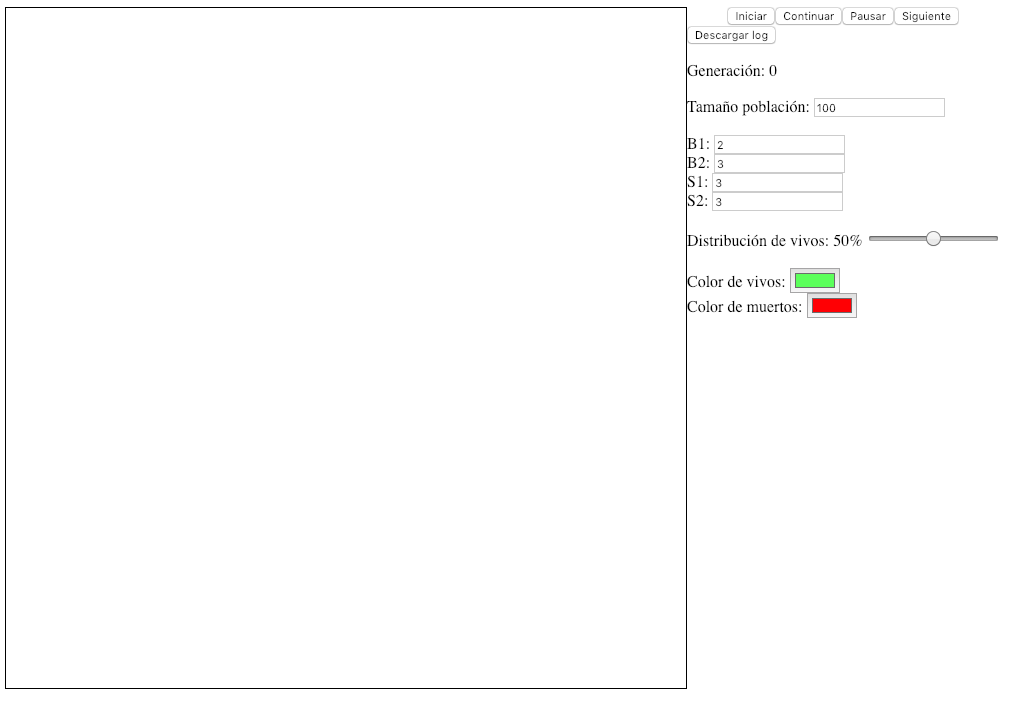
\includegraphics[scale=.3]{GOL/img/interfaz.png}
			\caption{Interfaz gráfica del programa}
			\label{fig:gol1}
		\end{center}
	\end{figure}

	\begin{figure}[H]
		\begin{center}
			
\includegraphics[scale=.5]{GOL/img/1.png}
			\caption{Prueba 1}
			\label{fig:gol2}
		\end{center}
	\end{figure}

	\begin{figure}[H]
		\begin{center}
			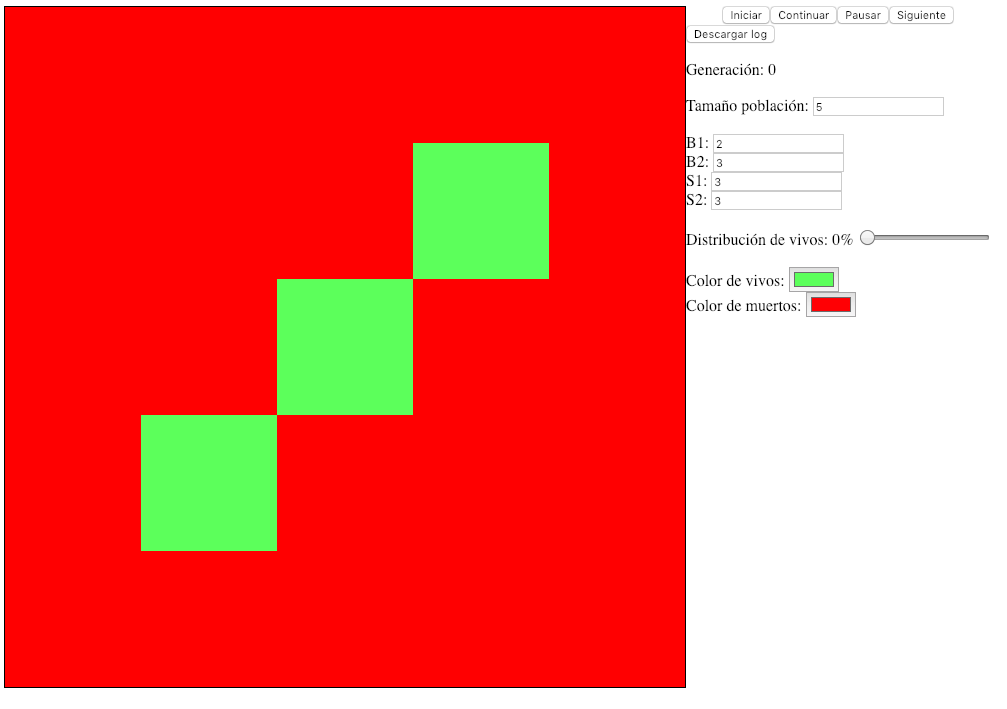
\includegraphics[scale=.3]{GOL/img/test1-1.png}
			\caption{Resultado para la prueba 1 (1)}
			\label{fig:gol3}
		\end{center}
	\end{figure}

	\begin{figure}[H]
		\begin{center}
			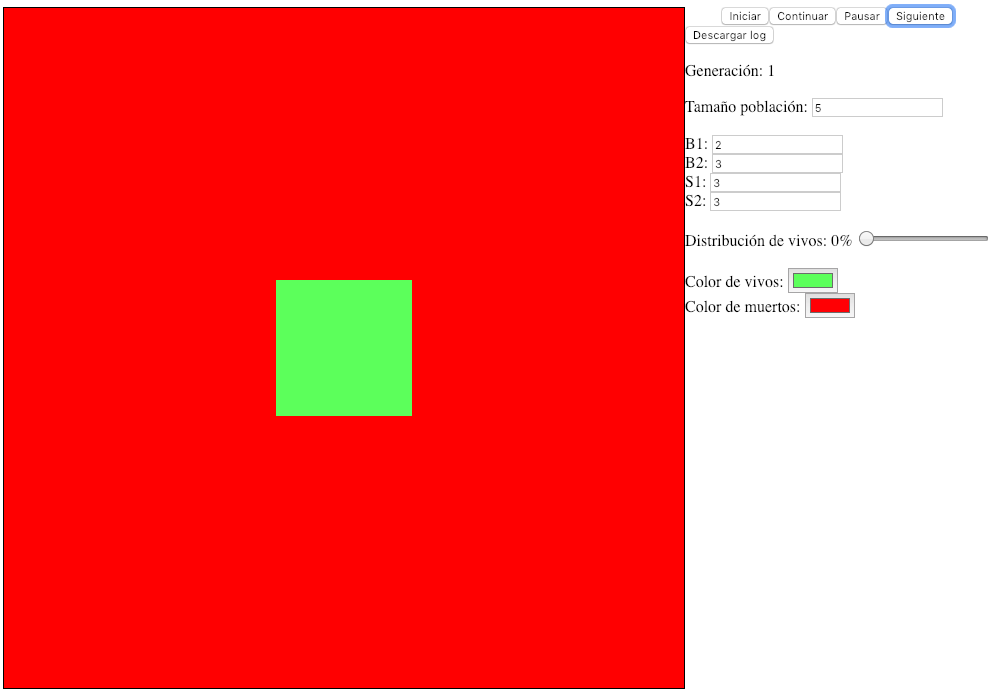
\includegraphics[scale=.3]{GOL/img/test1-2.png}
			\caption{Resultado para la prueba 1 (2)}
			\label{fig:gol4}
		\end{center}
	\end{figure}

	\begin{figure}[H]
		\begin{center}
			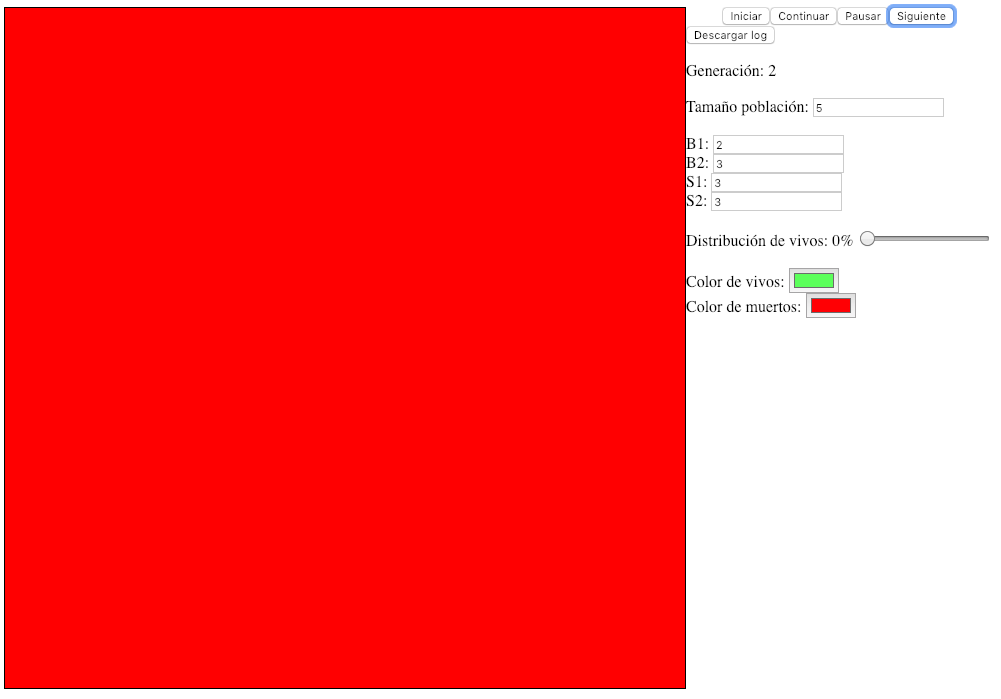
\includegraphics[scale=.3]{GOL/img/test1-3.png}
			\caption{Resultado para la prueba 1 (3)}
			\label{fig:gol5}
		\end{center}
	\end{figure}

	\begin{figure}[H]
		\begin{center}
			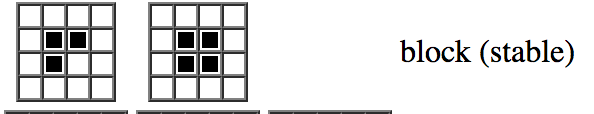
\includegraphics[scale=.5]{GOL/img/2.png}
			\caption{Prueba 2}
			\label{fig:gol4}
		\end{center}
	\end{figure}

	\begin{figure}[H]
		\begin{center}
			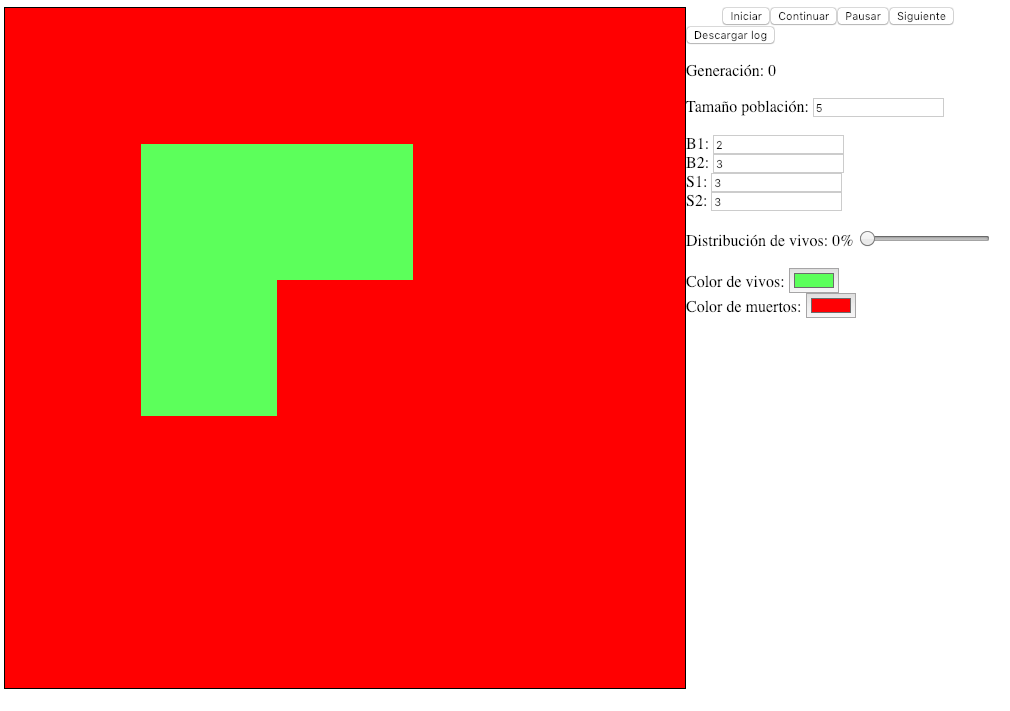
\includegraphics[scale=.3]{GOL/img/test2-1.png}
			\caption{Resultado para la prueba 2 (1)}
			\label{fig:gol5}
		\end{center}
	\end{figure}

	\begin{figure}[H]
		\begin{center}
			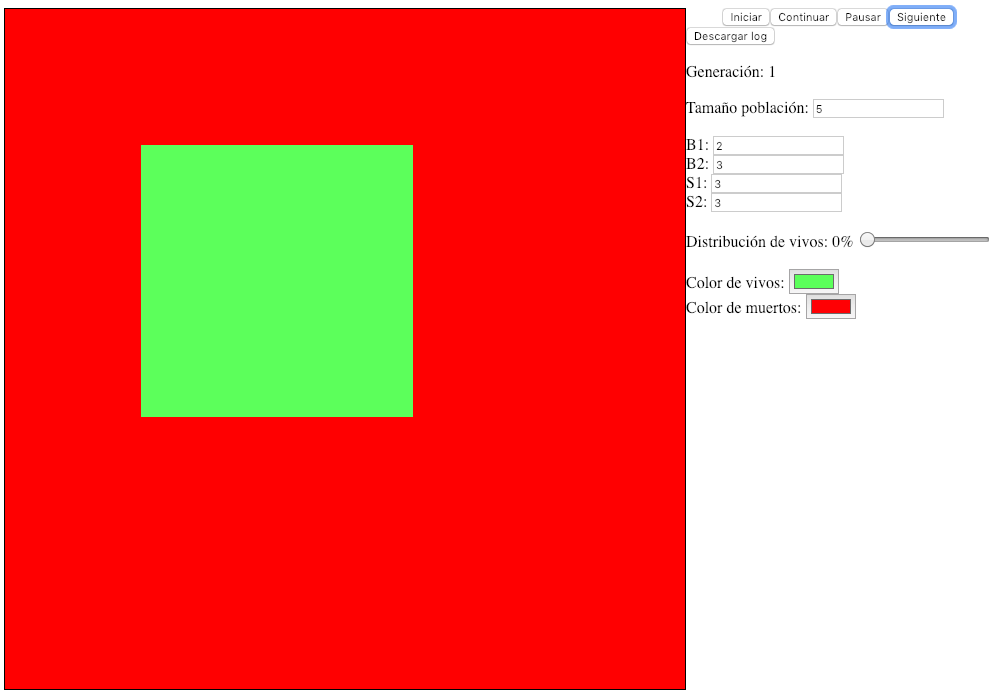
\includegraphics[scale=.3]{GOL/img/test2-2.png}
			\caption{Resultado para la prueba 2 (2)}
			\label{fig:gol4}
		\end{center}
	\end{figure}

	\begin{figure}[H]
		\begin{center}
			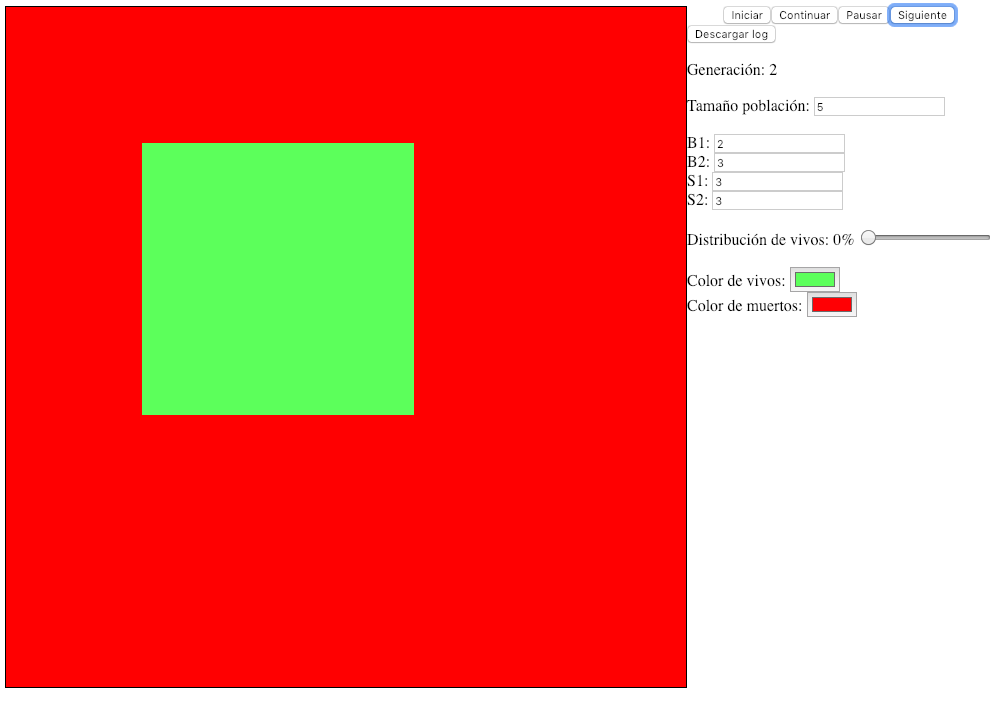
\includegraphics[scale=.3]{GOL/img/test2-3.png}
			\caption{Resultado para la prueba 2 (3)}
			\label{fig:gol5}
		\end{center}
	\end{figure}

	\begin{figure}[H]
		\begin{center}
			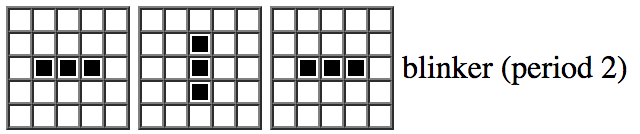
\includegraphics[scale=.5]{GOL/img/3.png}
			\caption{Prueba 3}
			\label{fig:gol4}
		\end{center}
	\end{figure}

	\begin{figure}[H]
		\begin{center}
			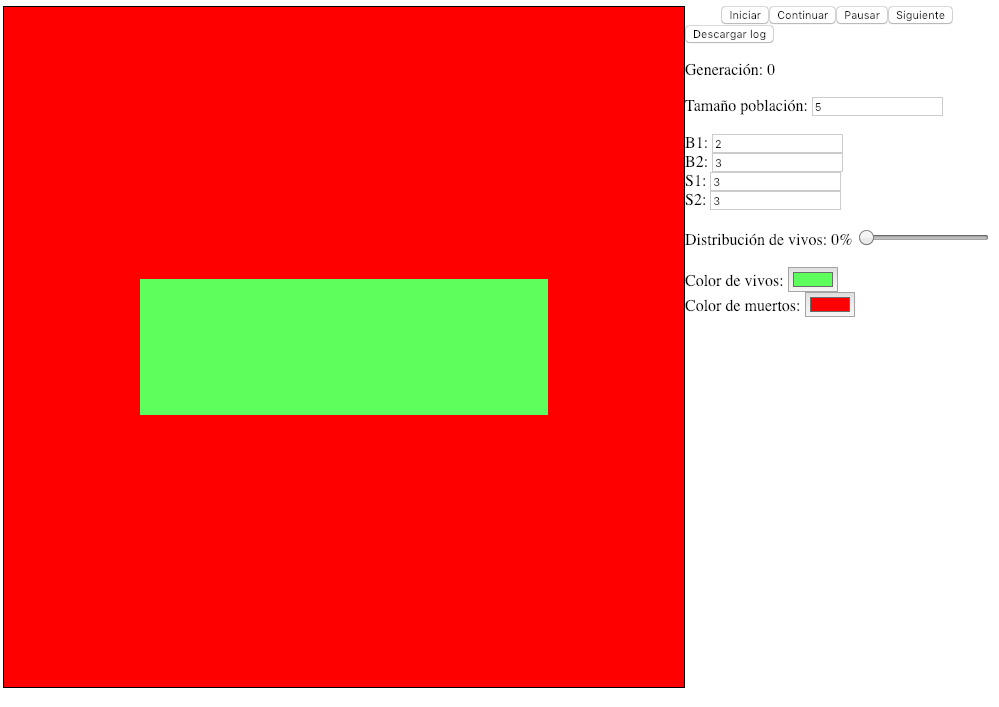
\includegraphics[scale=.3]{GOL/img/test3-1.png}
			\caption{Resultado para la prueba 3 (1)}
			\label{fig:gol5}
		\end{center}
	\end{figure}

	\begin{figure}[H]
		\begin{center}
			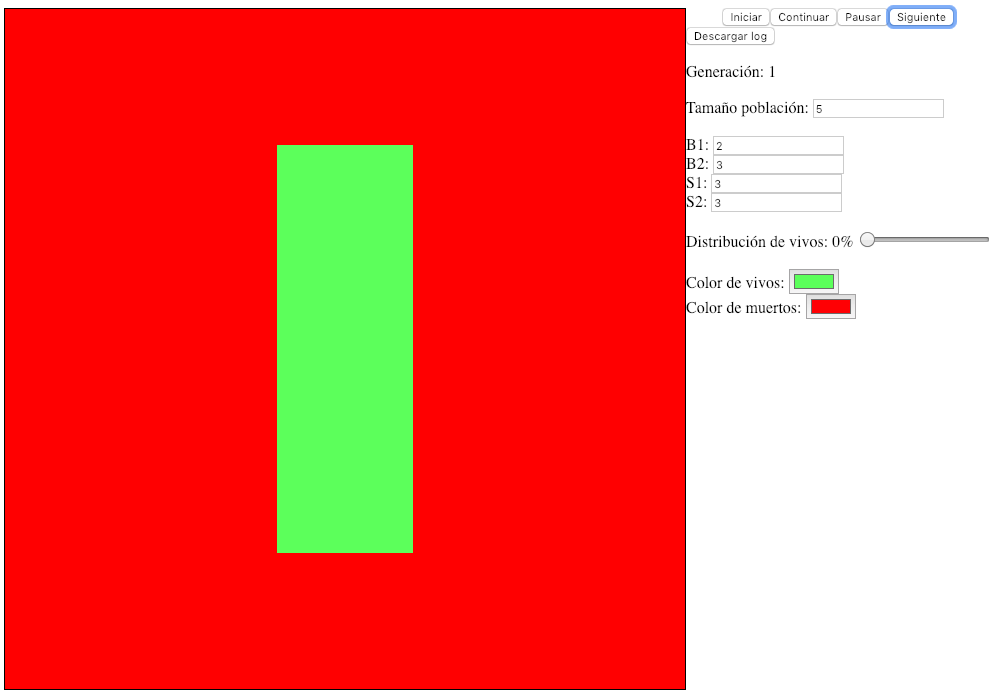
\includegraphics[scale=.3]{GOL/img/test3-2.png}
			\caption{Resultado para la prueba 3 (2)}
			\label{fig:gol4}
		\end{center}
	\end{figure}

	\begin{figure}[H]
		\begin{center}
			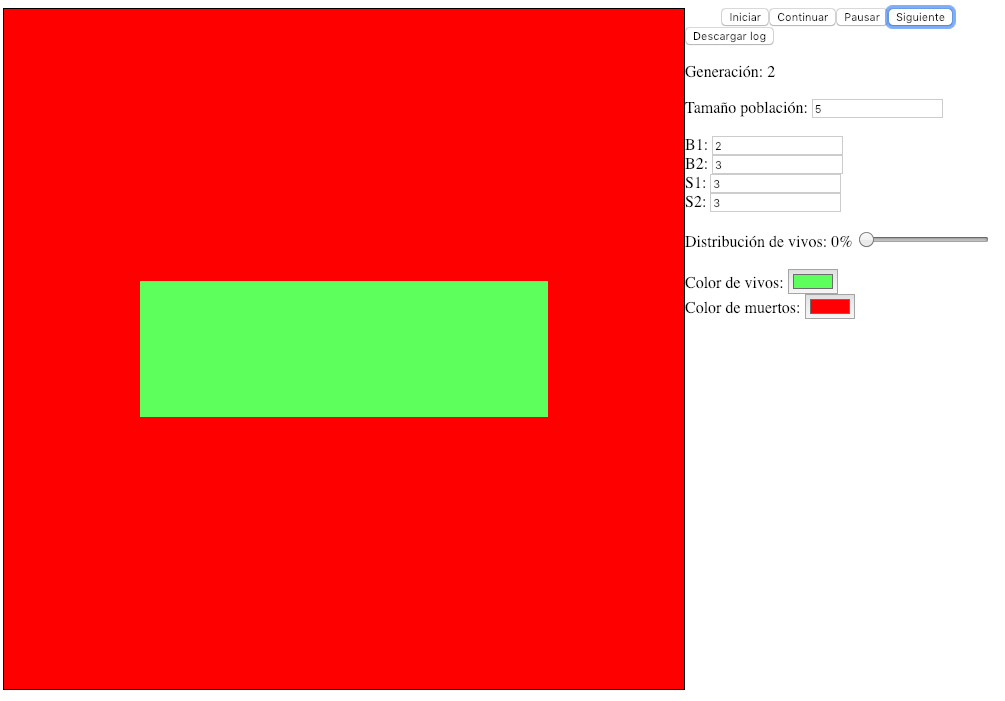
\includegraphics[scale=.3]{GOL/img/test3-3.png}
			\caption{Resultado para la prueba 3 (3)}
			\label{fig:gol5}
		\end{center}
	\end{figure}

	\begin{figure}[H]
		\begin{center}
			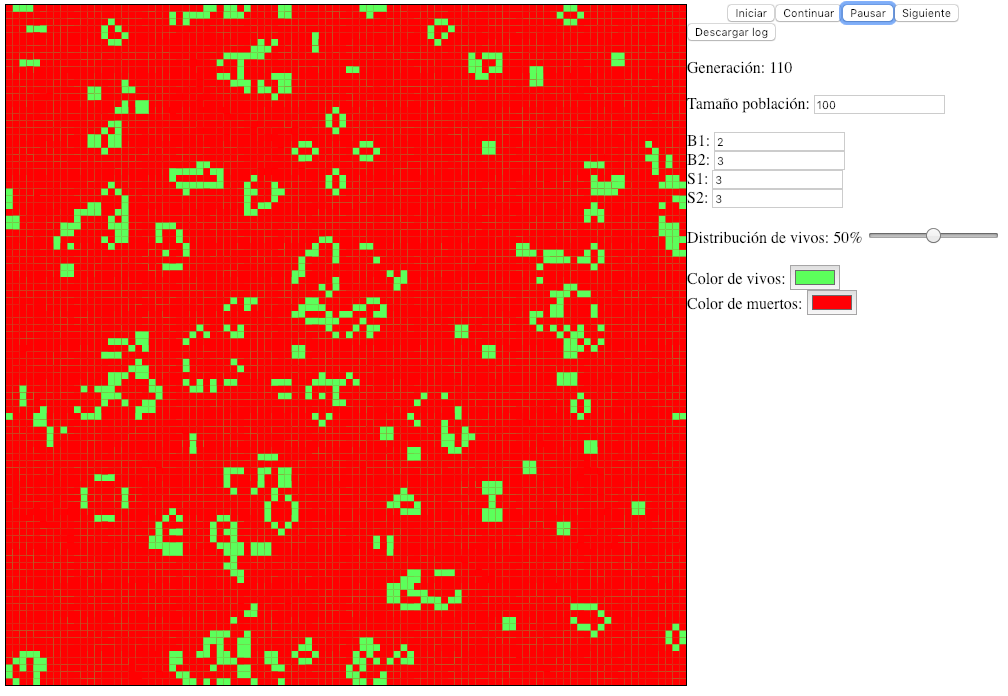
\includegraphics[scale=.3]{GOL/img/life1.png}
			\caption{Juego de la vida después de 100 generaciones}
			\label{fig:gol5}
		\end{center}
	\end{figure}

	\begin{figure}[H]
		\begin{center}
			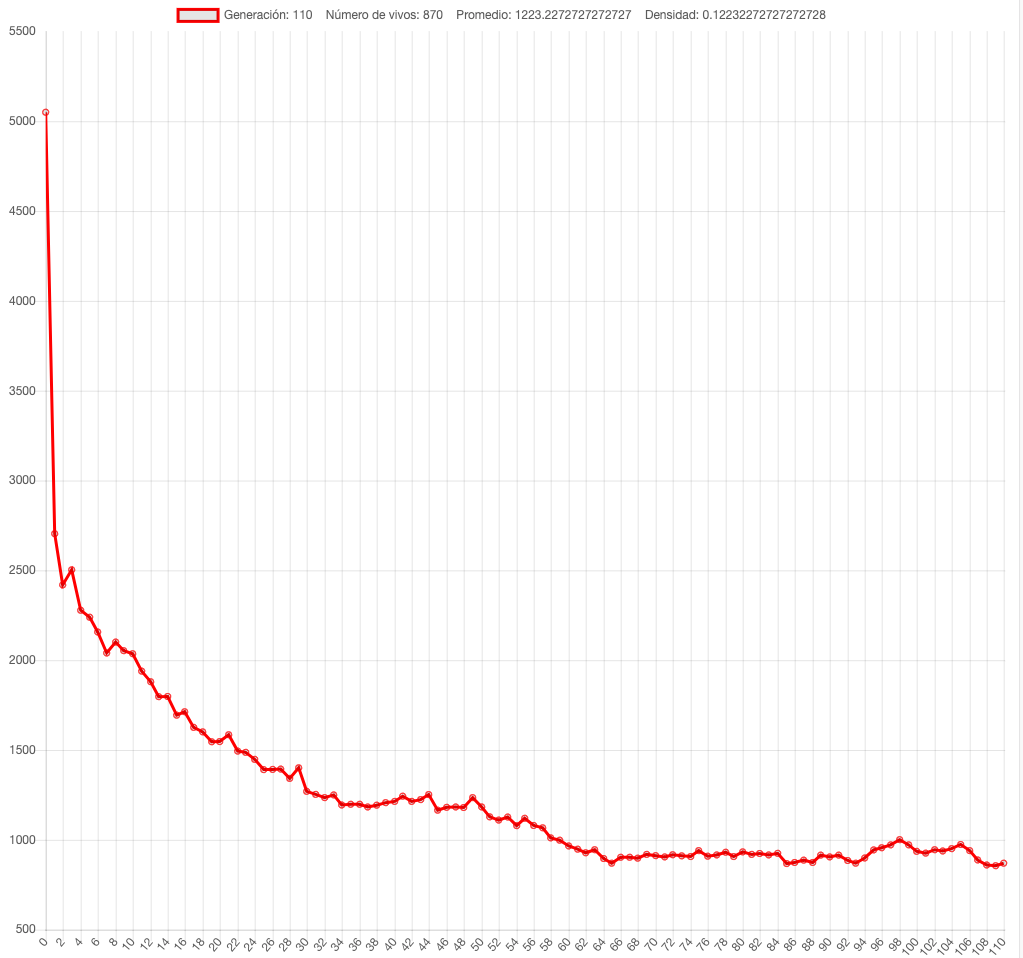
\includegraphics[scale=.24]{GOL/img/life2.png}
			\caption{Total células vivas en juego de la vida después de 100 generaciones}
			\label{fig:gol5}
		\end{center}
	\end{figure}

	\begin{figure}[H]
		\begin{center}
			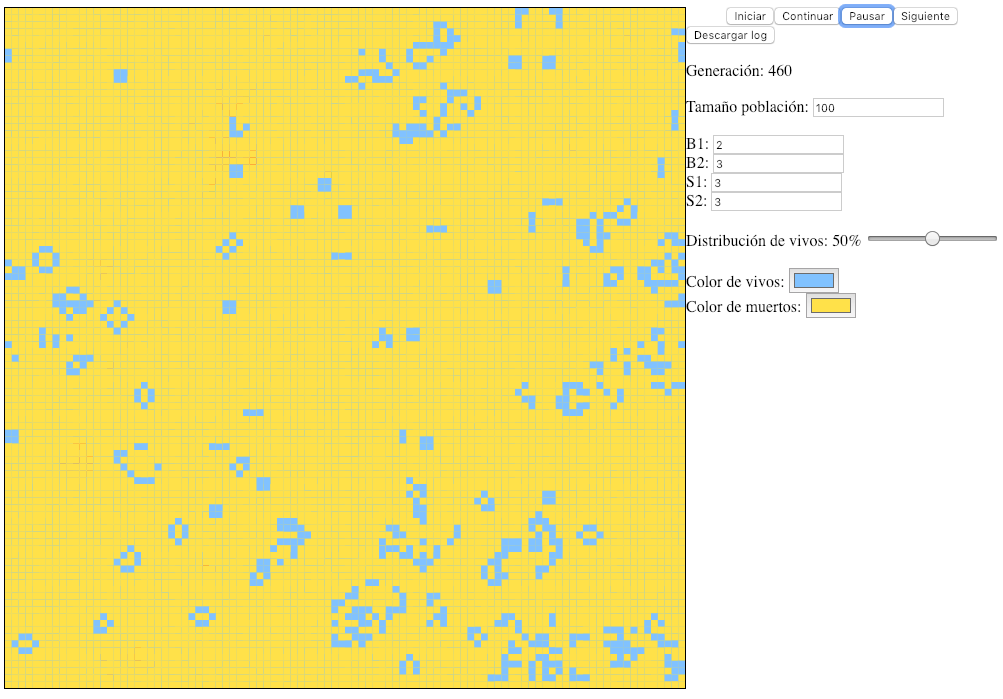
\includegraphics[scale=.3]{GOL/img/lifecolores.png}
			\caption{Juego de la vida con distintos colores}
			\label{fig:gol5}
		\end{center}
	\end{figure}

	\begin{figure}[H]
		\begin{center}
			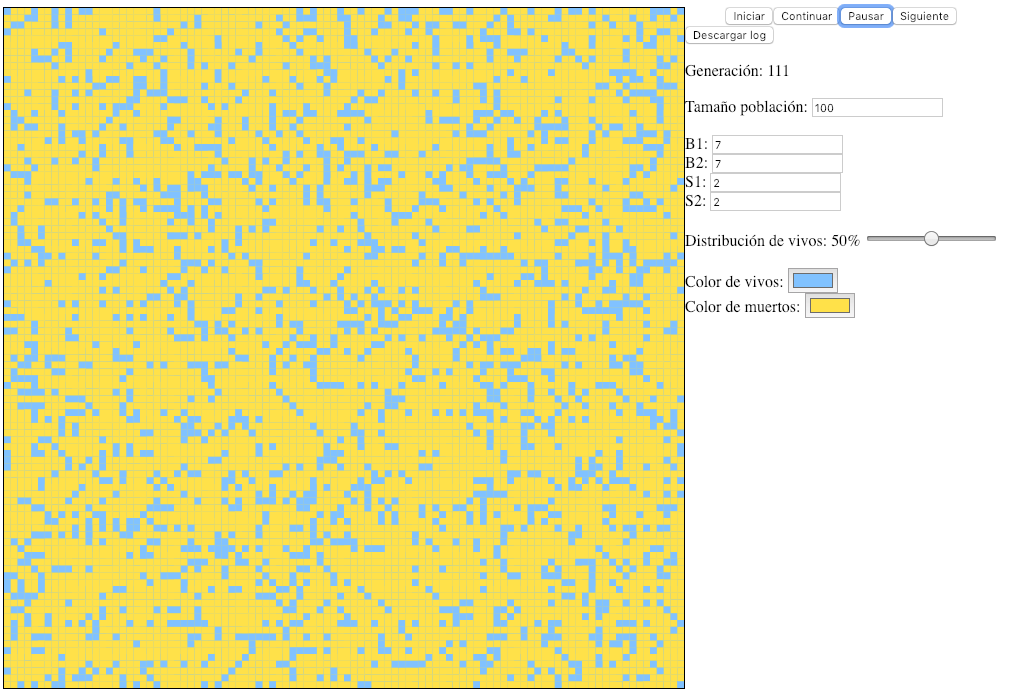
\includegraphics[scale=.3]{GOL/img/difusion1.png}
			\caption{Regla de difusión después de 100 generaciones}
			\label{fig:gol5}
		\end{center}
	\end{figure}

	\begin{figure}[H]
		\begin{center}
			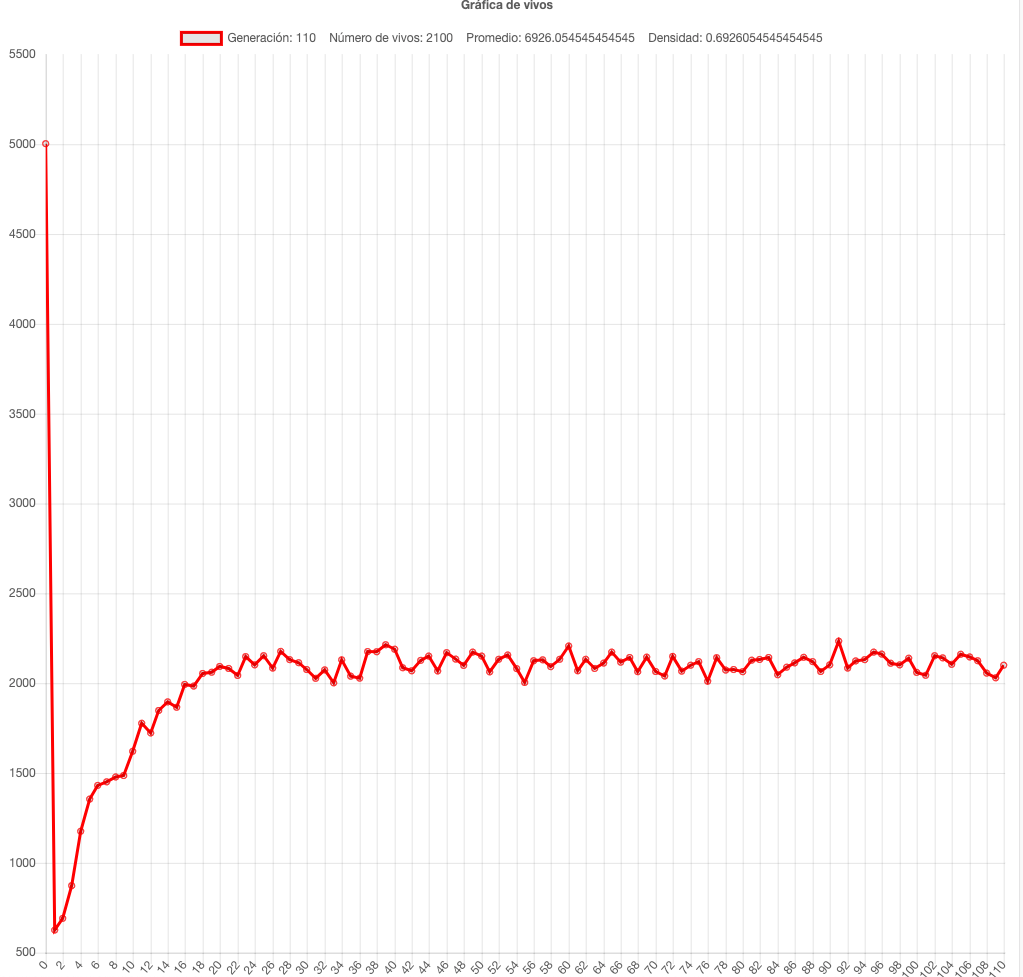
\includegraphics[scale=.24]{GOL/img/difusion2.png}
			\caption{Total células vivas con regla difusión después de 100 generaciones}
			\label{fig:gol5}
		\end{center}
	\end{figure}

\subsubsection{Análisis de poblaciones}
	En esta parte se hicieron pruebas con la regla de life y difusión aumentando la densidad de la población de 10 en 10 por ciento hasta llegar al máximo de 90 por ciento debido que en un 100 por ciento no se aprecia nada al igual que en cero, las pruebas de realizaron tras 1000 generaciones en una matriz de 100 por 100.

	\begin{figure}[H]
		\begin{center}
			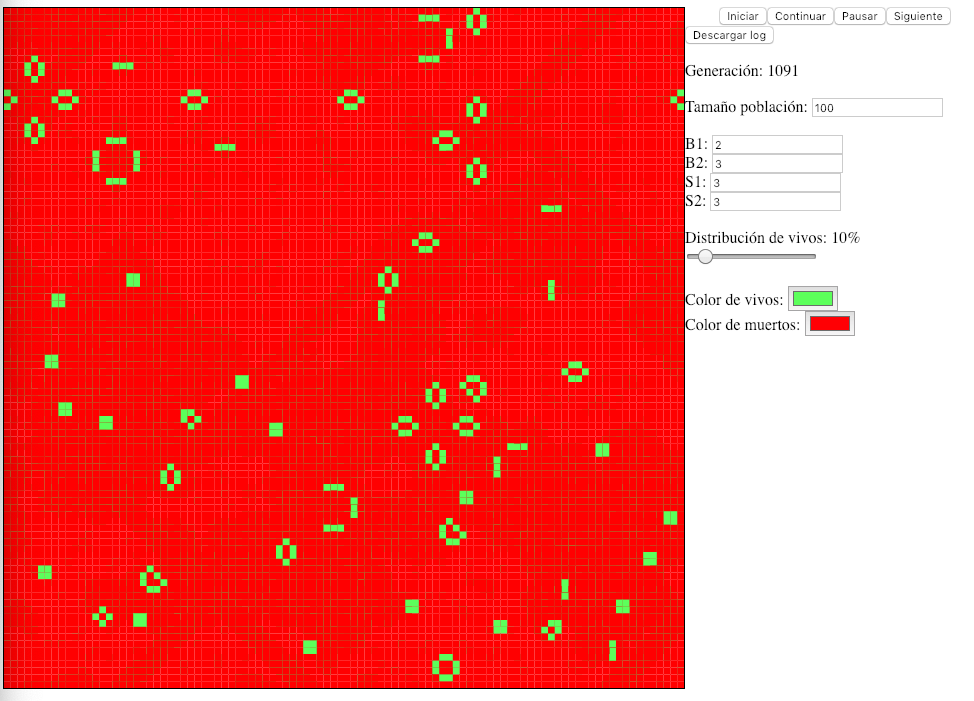
\includegraphics[scale=.3]{GOL/img/life10-1.png}
			\caption{Regla de life con probabilidad de 10\%}
			\label{fig:gol5}
		\end{center}
	\end{figure}

	\begin{figure}[H]
		\begin{center}
			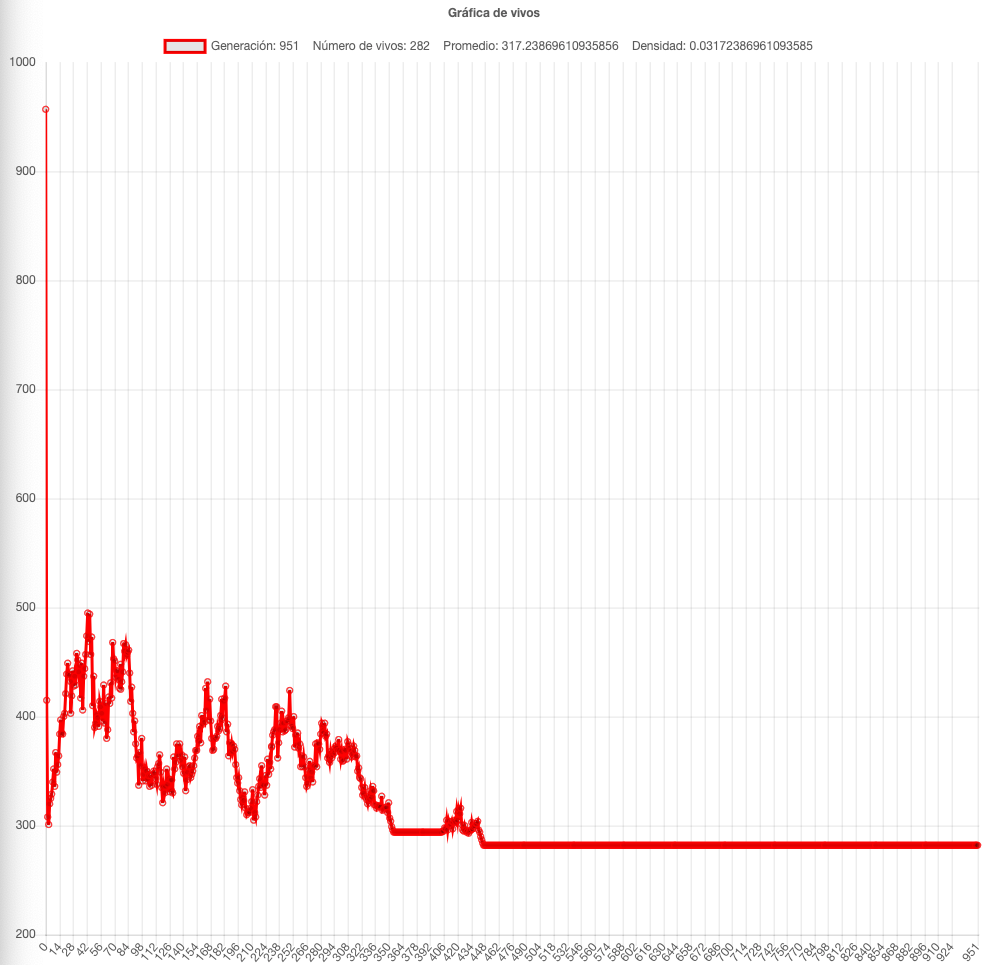
\includegraphics[scale=.24]{GOL/img/life10-2.png}
			\caption{Comportamiento de la población de la simulación anterior}
			\label{fig:gol5}
		\end{center}
	\end{figure}

	\begin{figure}[H]
		\begin{center}
			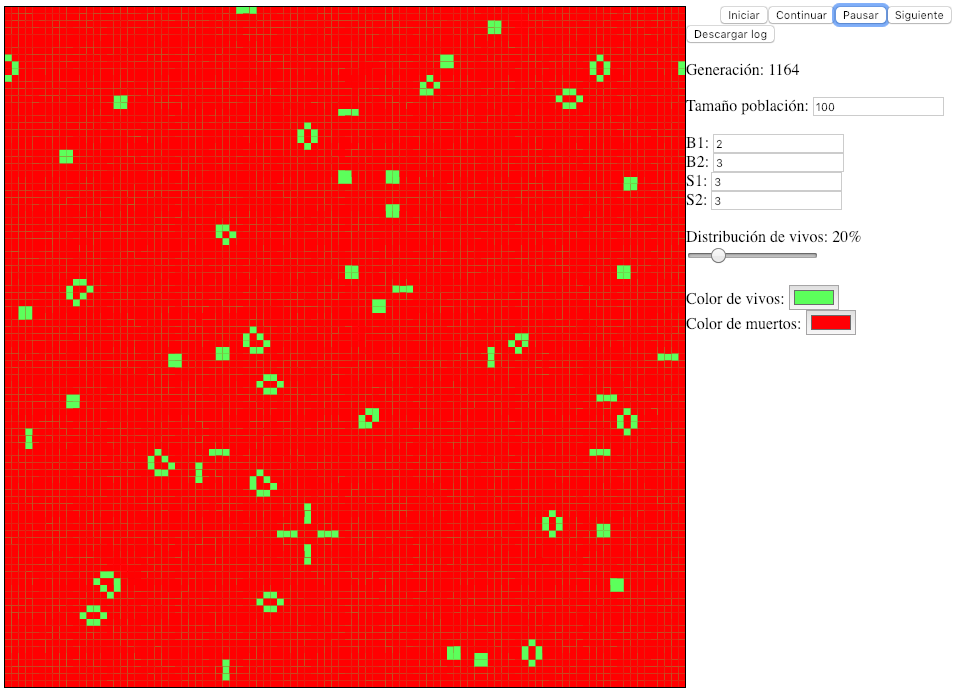
\includegraphics[scale=.3]{GOL/img/life20-1.png}
			\caption{Regla de life con probabilidad de 20\%}
			\label{fig:gol5}
		\end{center}
	\end{figure}

	\begin{figure}[H]
		\begin{center}
			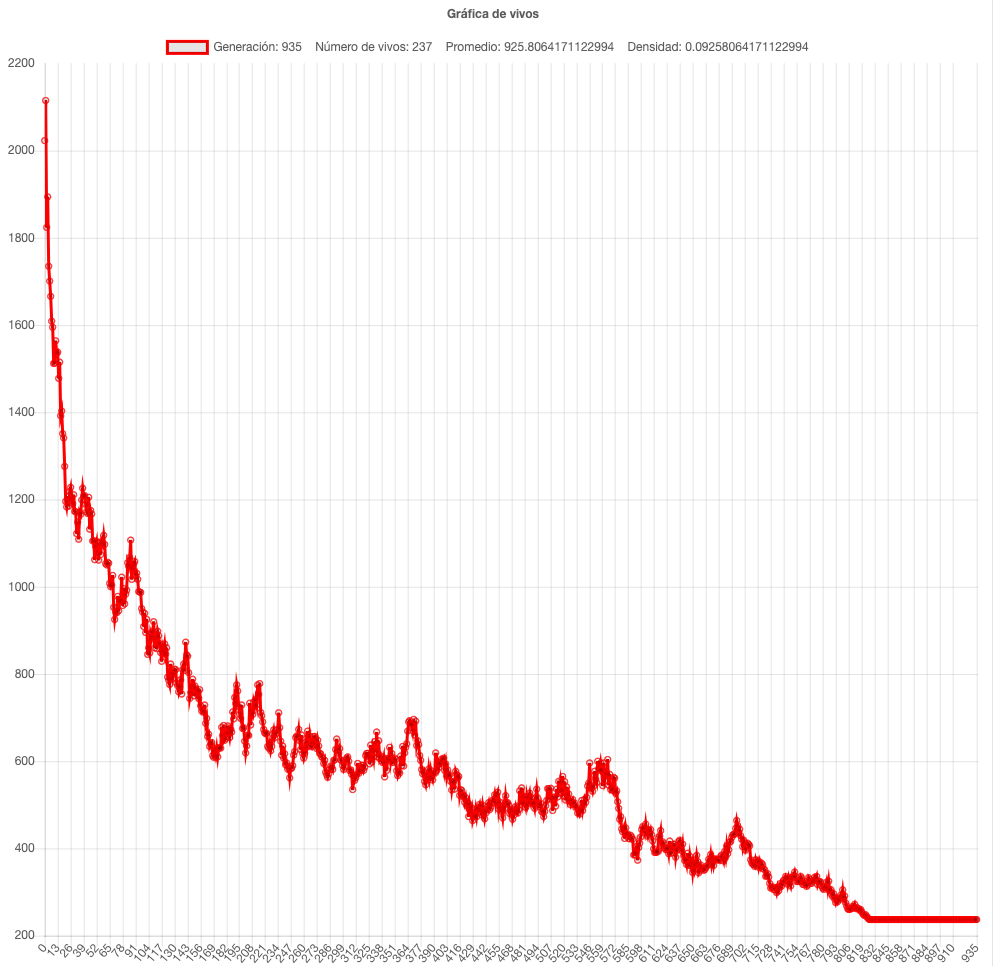
\includegraphics[scale=.24]{GOL/img/life20-2.png}
			\caption{Comportamiento de la población de la simulación anterior}
			\label{fig:gol5}
		\end{center}
	\end{figure}

	\begin{figure}[H]
		\begin{center}
			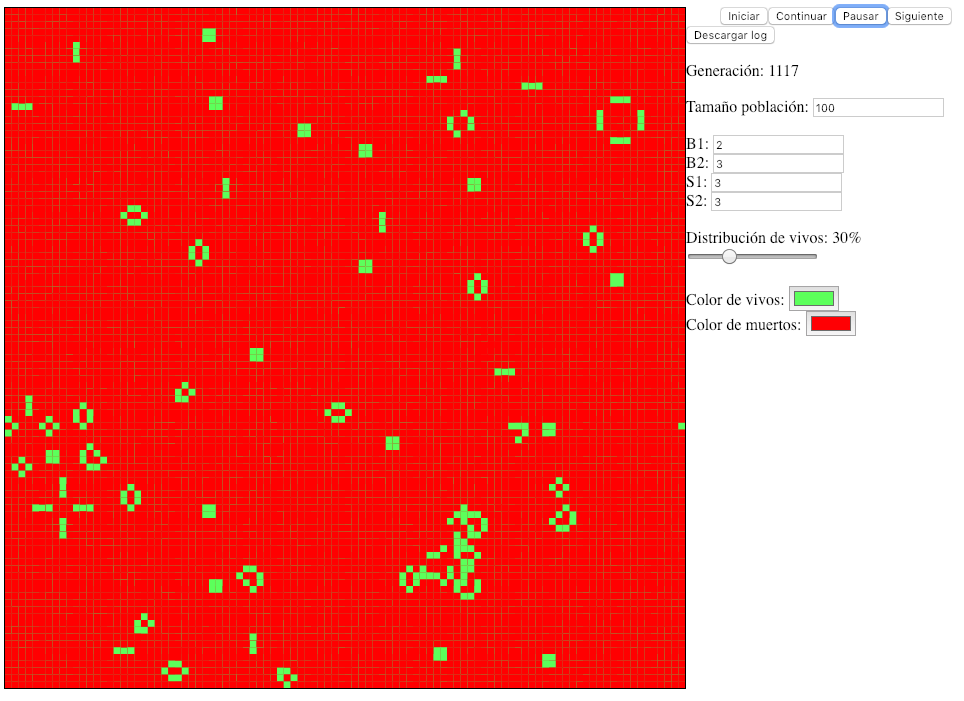
\includegraphics[scale=.3]{GOL/img/life30-1.png}
			\caption{Regla de life con probabilidad de 30\%}
			\label{fig:gol5}
		\end{center}
	\end{figure}

	\begin{figure}[H]
		\begin{center}
			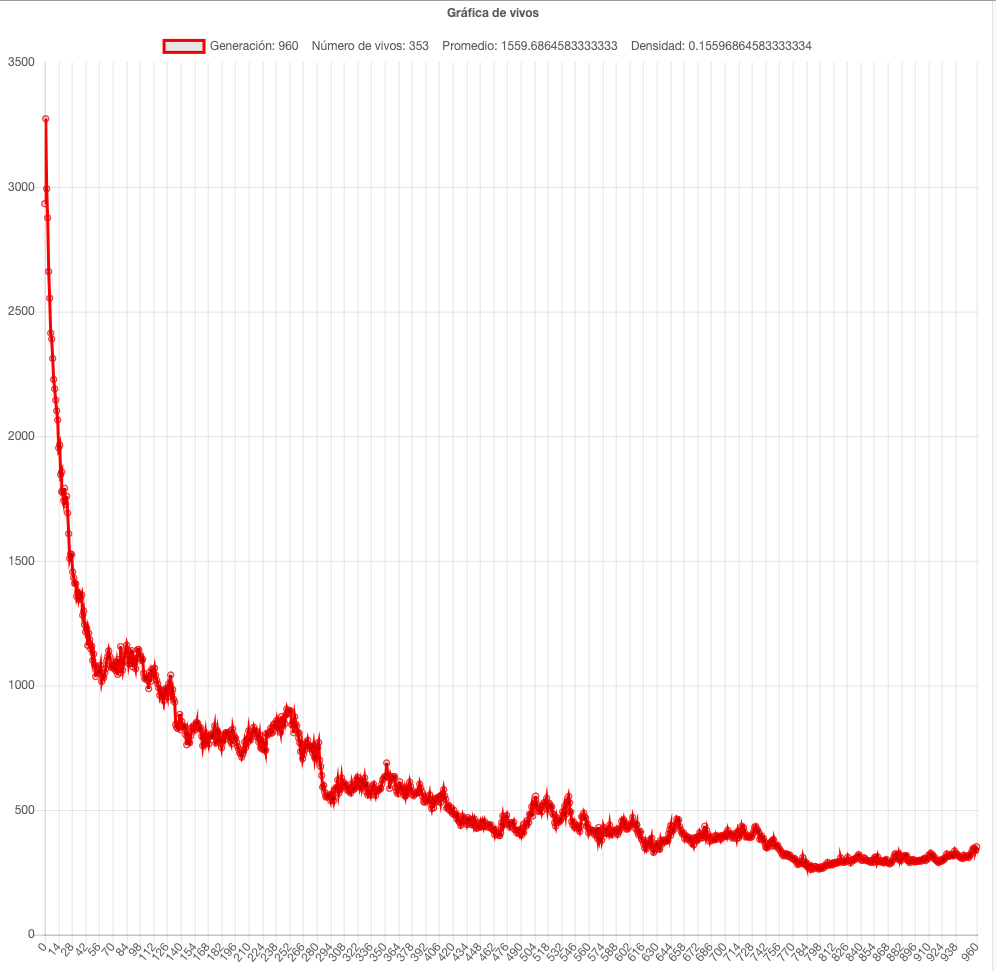
\includegraphics[scale=.24]{GOL/img/life30-2.png}
			\caption{Comportamiento de la población de la simulación anterior}
			\label{fig:gol5}
		\end{center}
	\end{figure}

	\begin{figure}[H]
		\begin{center}
			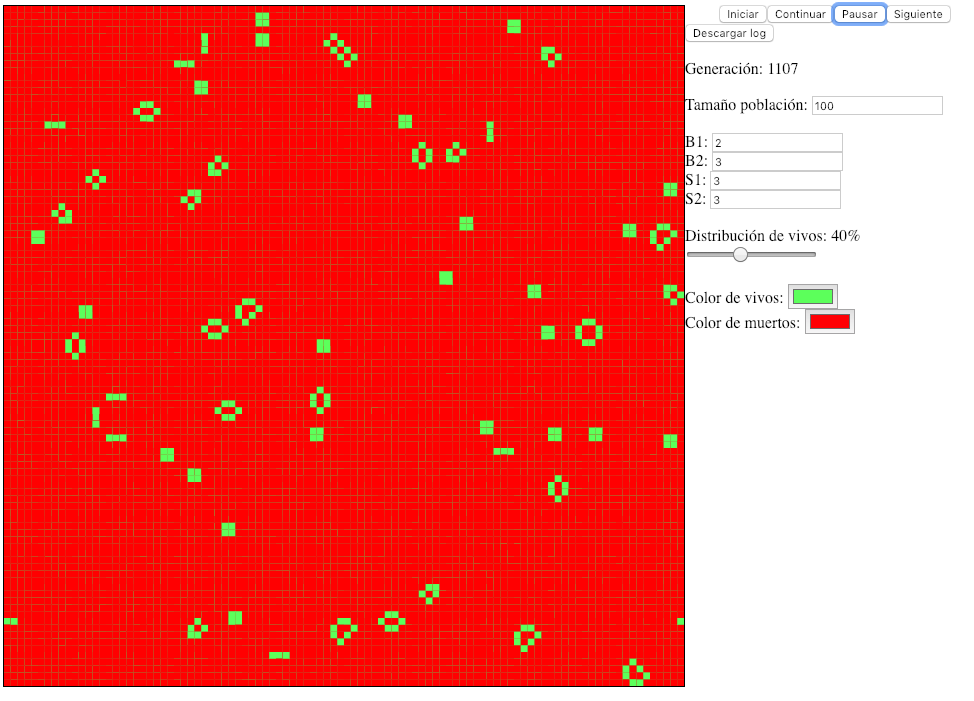
\includegraphics[scale=.3]{GOL/img/life40-1.png}
			\caption{Regla de life con probabilidad de 40\%}
			\label{fig:gol5}
		\end{center}
	\end{figure}

	\begin{figure}[H]
		\begin{center}
			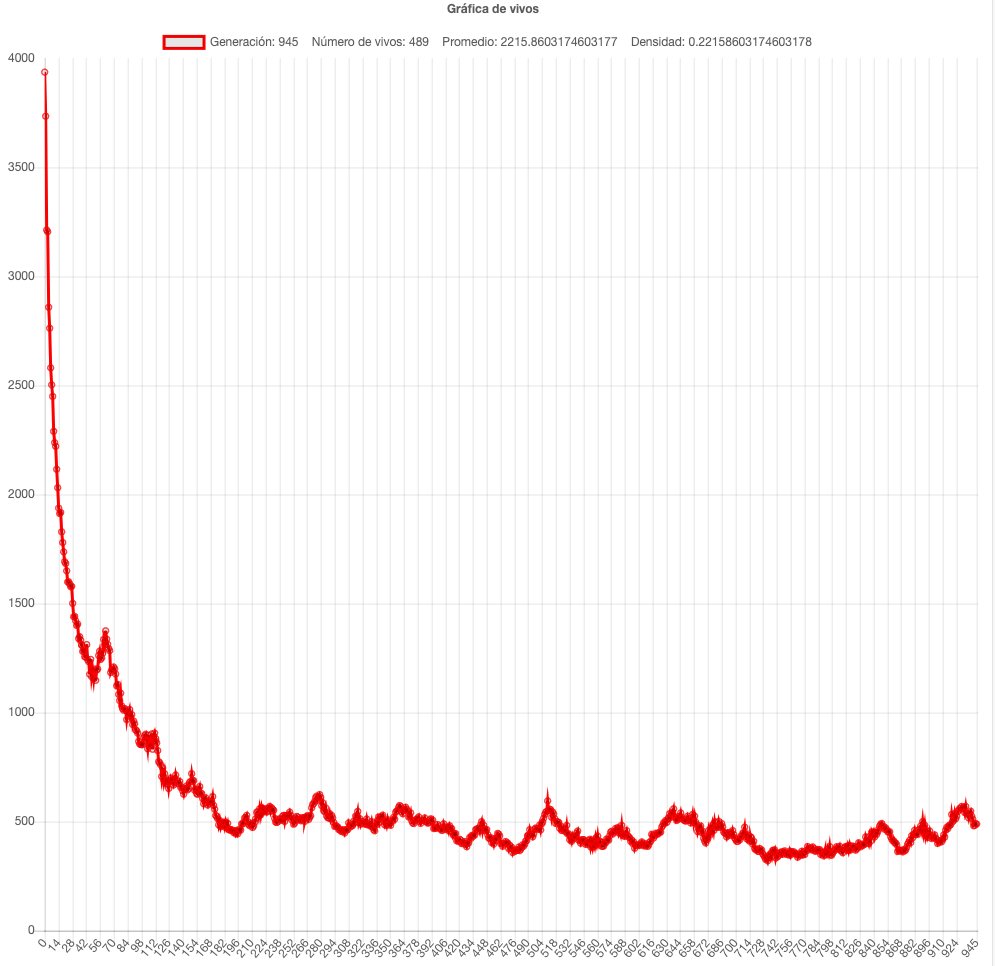
\includegraphics[scale=.24]{GOL/img/life40-2.png}
			\caption{Comportamiento de la población de la simulación anterior}
			\label{fig:gol5}
		\end{center}
	\end{figure}

	\begin{figure}[H]
		\begin{center}
			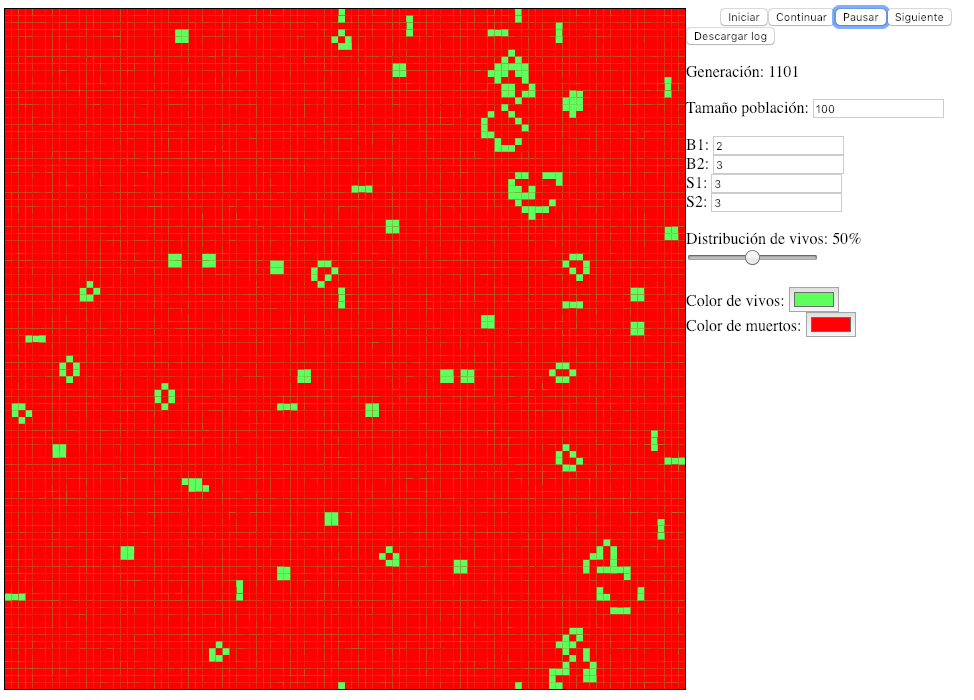
\includegraphics[scale=.3]{GOL/img/life50-1.png}
			\caption{Regla de life con probabilidad de 50\%}
			\label{fig:gol5}
		\end{center}
	\end{figure}

	\begin{figure}[H]
		\begin{center}
			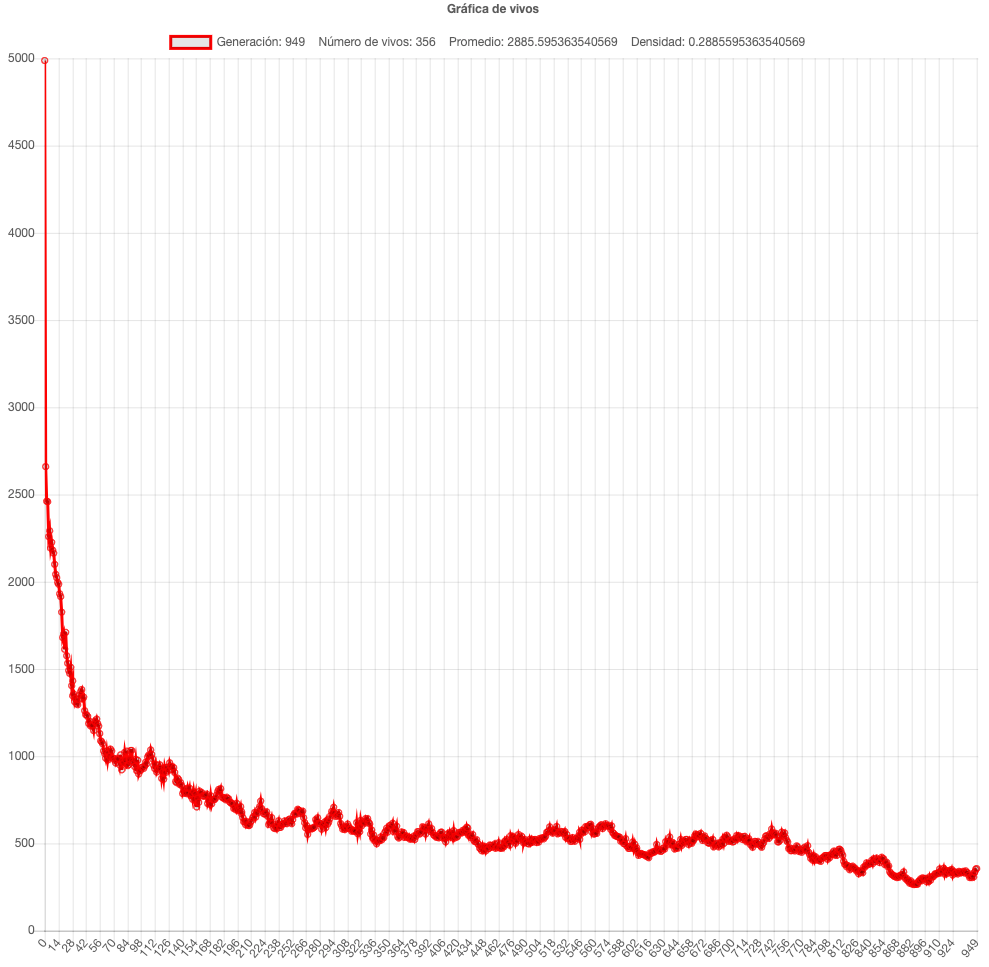
\includegraphics[scale=.24]{GOL/img/life50-2.png}
			\caption{Comportamiento de la población de la simulación anterior}
			\label{fig:gol5}
		\end{center}
	\end{figure}

	\begin{figure}[H]
		\begin{center}
			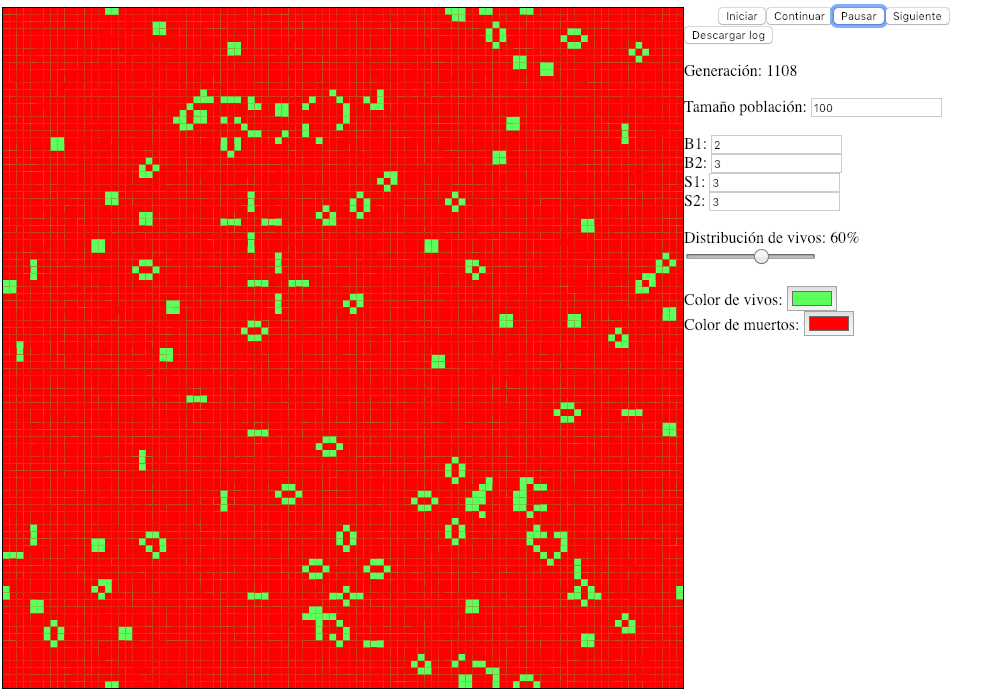
\includegraphics[scale=.3]{GOL/img/life60-1.png}
			\caption{Regla de life con probabilidad de 60\%}
			\label{fig:gol5}
		\end{center}
	\end{figure}

	\begin{figure}[H]
		\begin{center}
			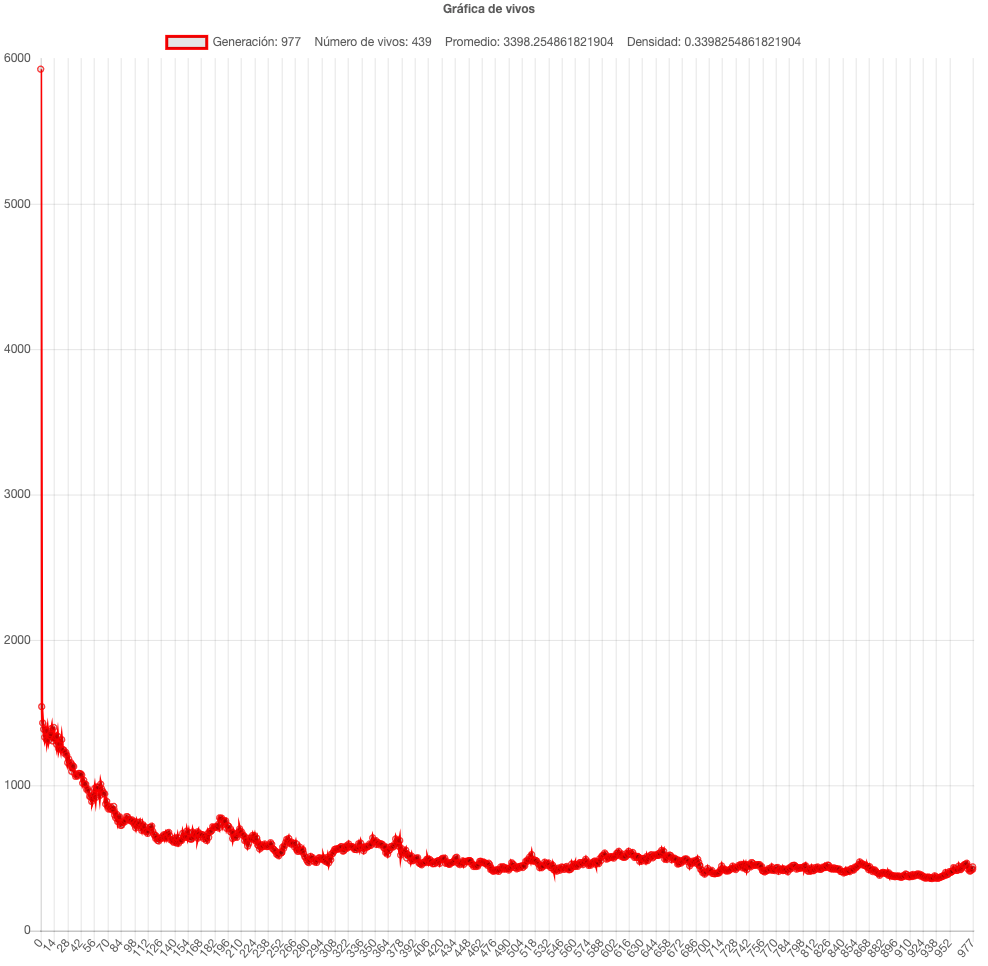
\includegraphics[scale=.24]{GOL/img/life60-2.png}
			\caption{Comportamiento de la población de la simulación anterior}
			\label{fig:gol5}
		\end{center}
	\end{figure}

	\begin{figure}[H]
		\begin{center}
			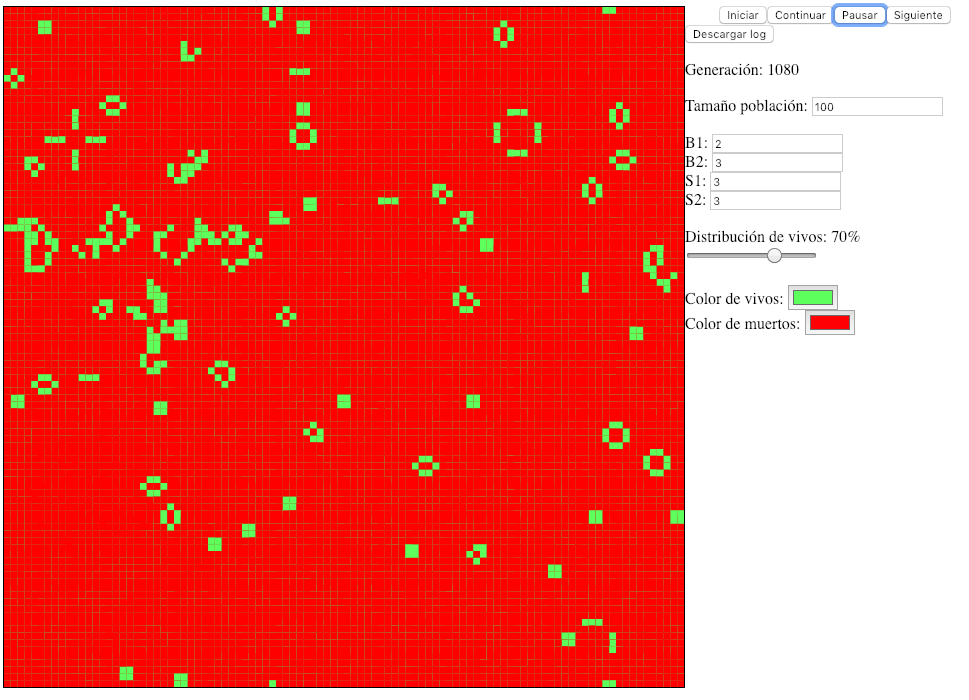
\includegraphics[scale=.3]{GOL/img/life70-1.png}
			\caption{Regla de life con probabilidad de 70\%}
			\label{fig:gol5}
		\end{center}
	\end{figure}

	\begin{figure}[H]
		\begin{center}
			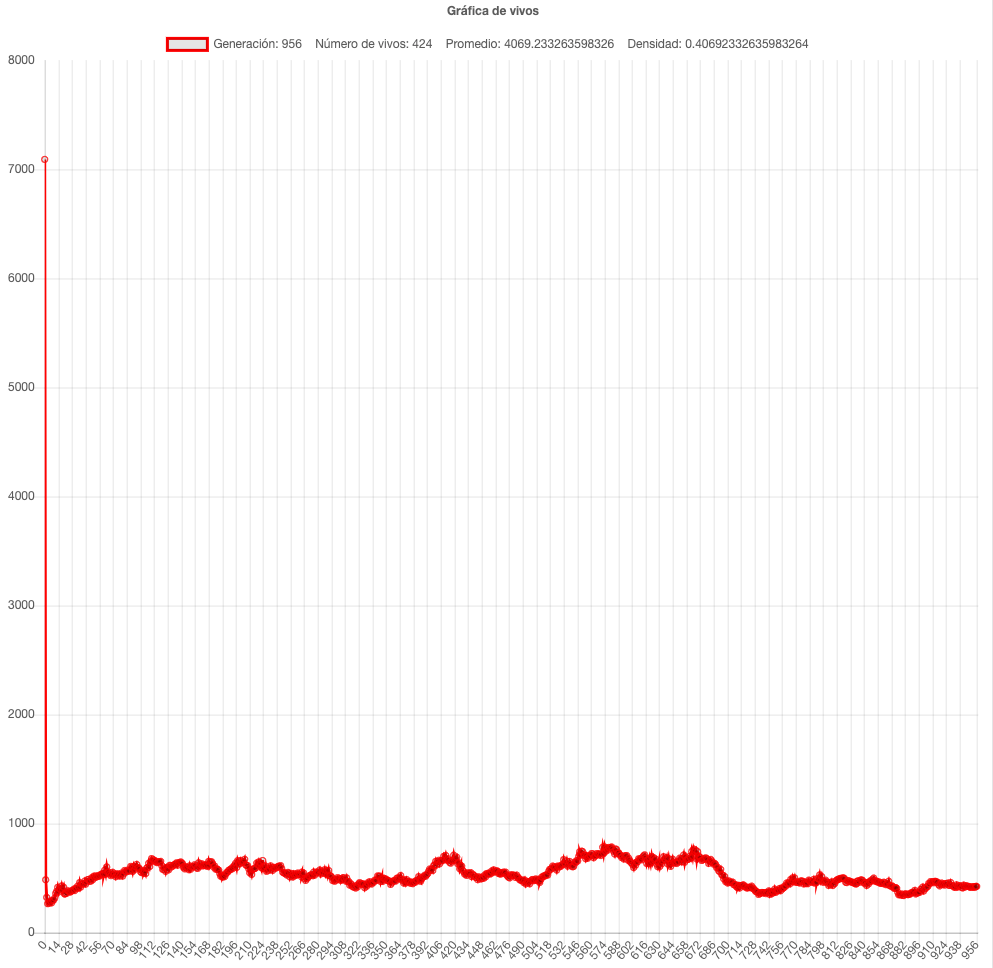
\includegraphics[scale=.24]{GOL/img/life70-2.png}
			\caption{Comportamiento de la población de la simulación anterior}
			\label{fig:gol5}
		\end{center}
	\end{figure}

	\begin{figure}[H]
		\begin{center}
			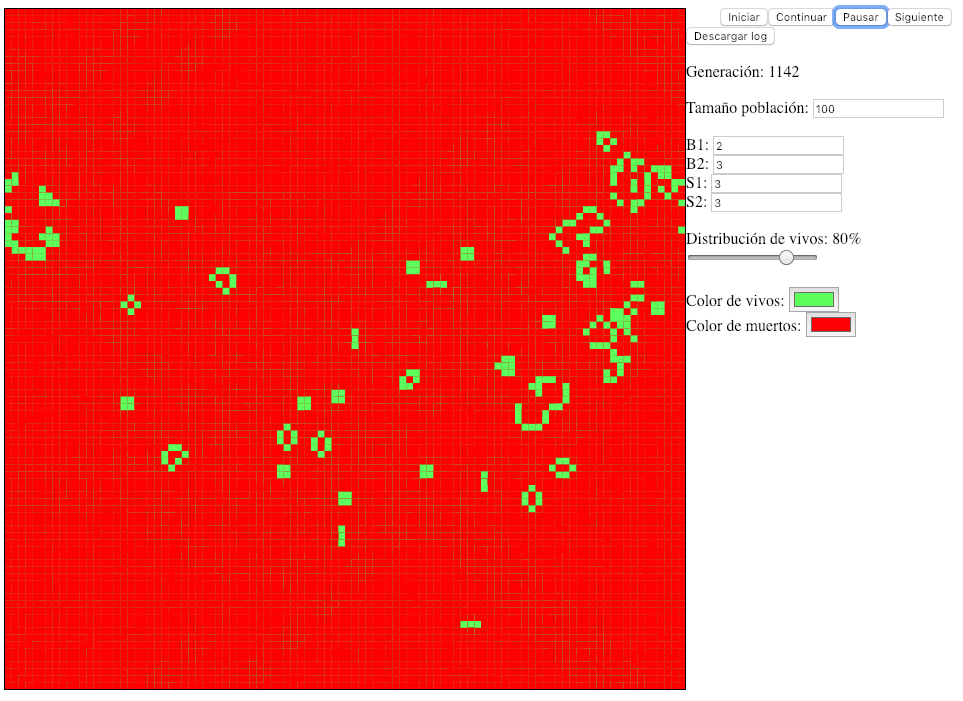
\includegraphics[scale=.3]{GOL/img/life80-1.png}
			\caption{Regla de life con probabilidad de 80\%}
			\label{fig:gol5}
		\end{center}
	\end{figure}

	\begin{figure}[H]
		\begin{center}
			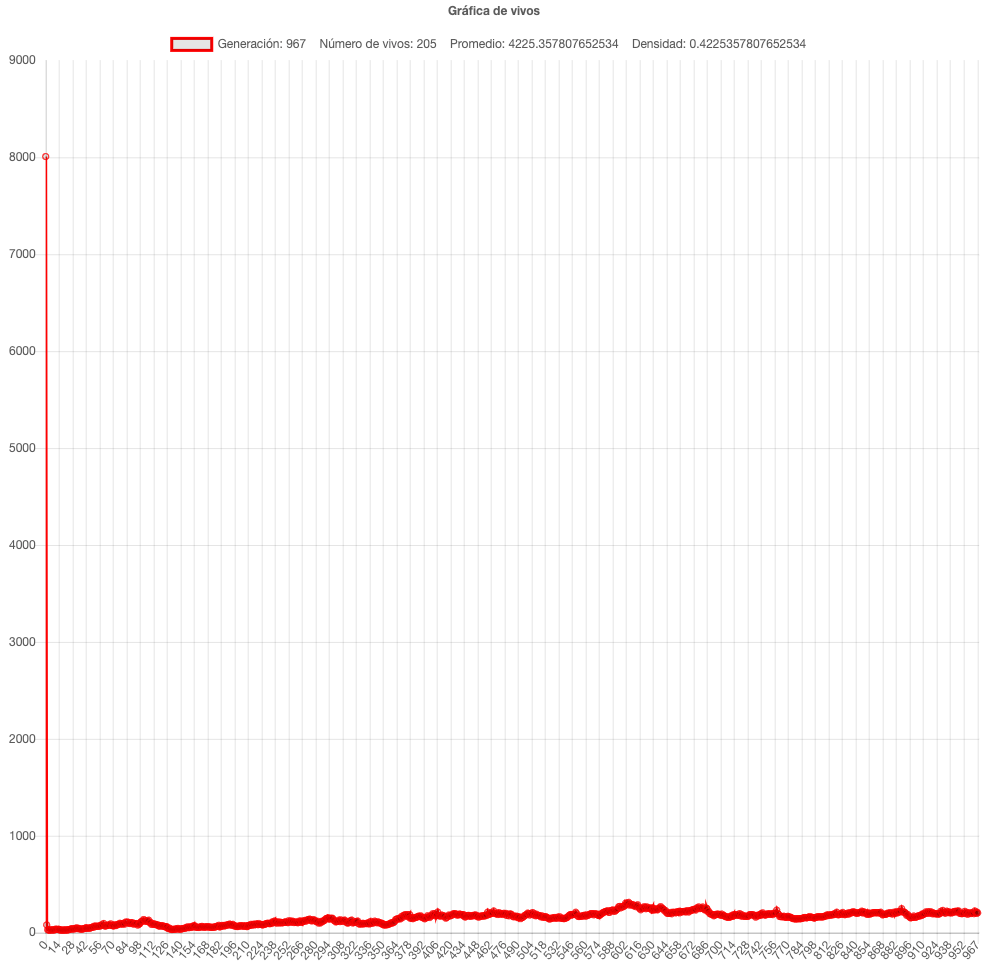
\includegraphics[scale=.24]{GOL/img/life80-2.png}
			\caption{Comportamiento de la población de la simulación anterior}
			\label{fig:gol5}
		\end{center}
	\end{figure}

	\begin{figure}[H]
		\begin{center}
			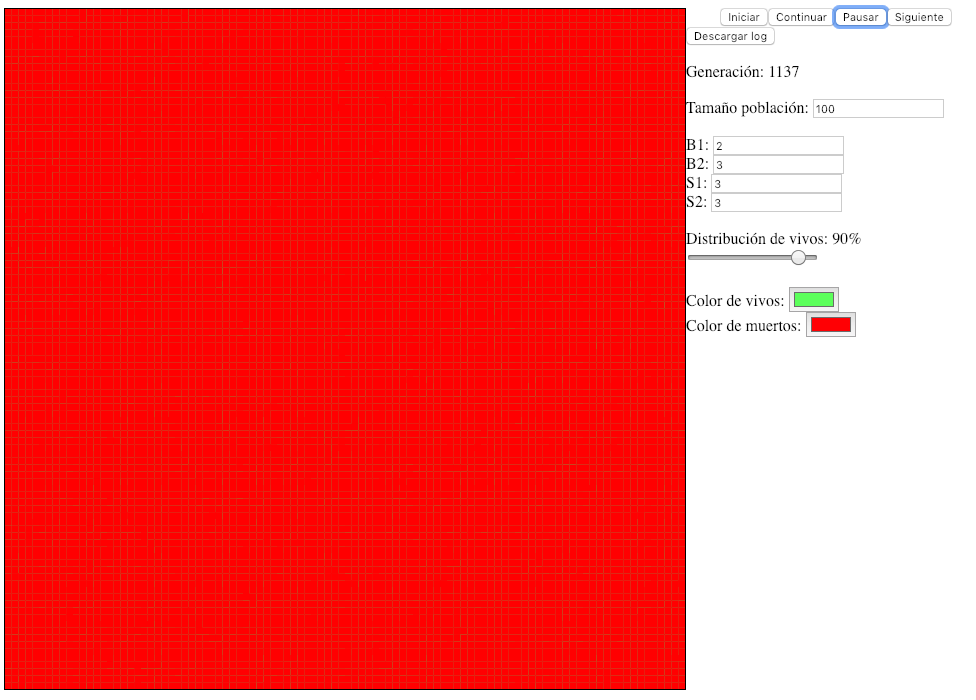
\includegraphics[scale=.3]{GOL/img/life90-1.png}
			\caption{Regla de life con probabilidad de 90\%}
			\label{fig:gol5}
		\end{center}
	\end{figure}

	\begin{figure}[H]
		\begin{center}
			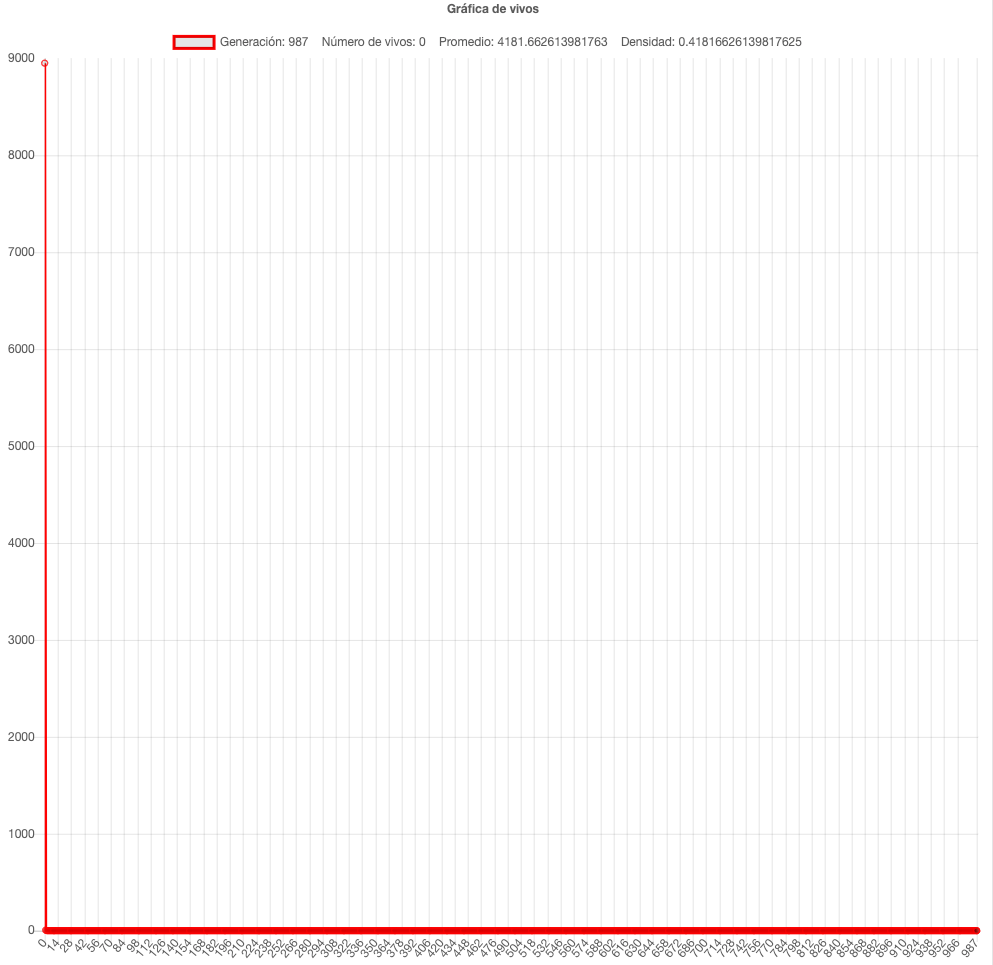
\includegraphics[scale=.24]{GOL/img/life90-2.png}
			\caption{Comportamiento de la población de la simulación anterior}
			\label{fig:gol5}
		\end{center}
	\end{figure}

	En todas las simulaciones se encuentra un comportamiento similar en el cual la población inicial es muy alta y de manera brusca disminuye y apartir de ahí decrece de manera lenta. En general, le regla de life hace que las poblaciones tiendan a una densidad de .03.

	\begin{figure}[H]
		\begin{center}
			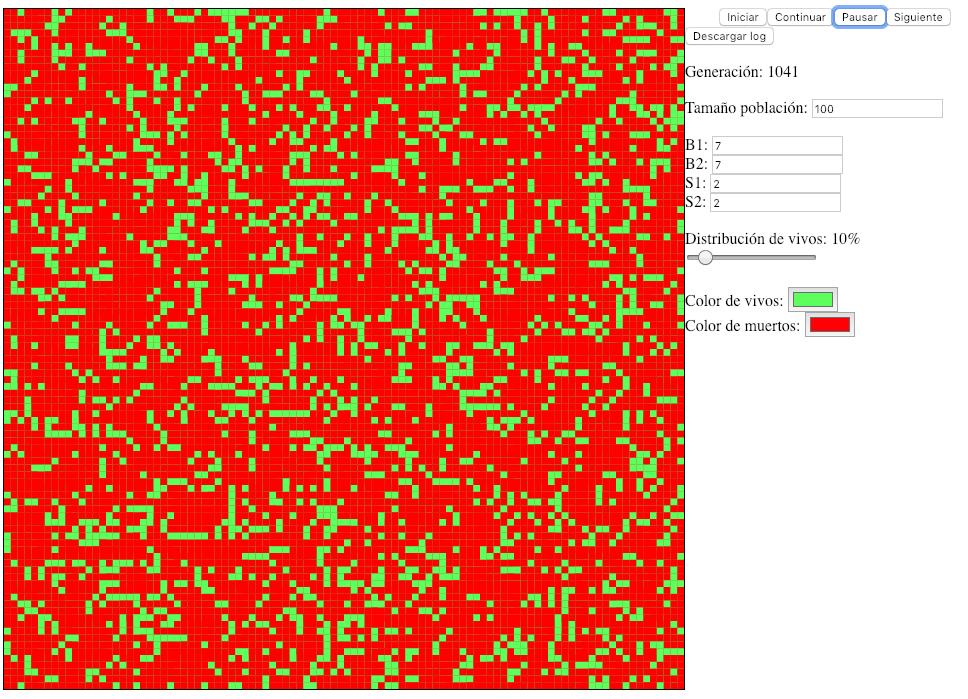
\includegraphics[scale=.3]{GOL/img/dif10-1.png}
			\caption{Regla de difusión con probabilidad de 10\%}
			\label{fig:gol5}
		\end{center}
	\end{figure}

	\begin{figure}[H]
		\begin{center}
			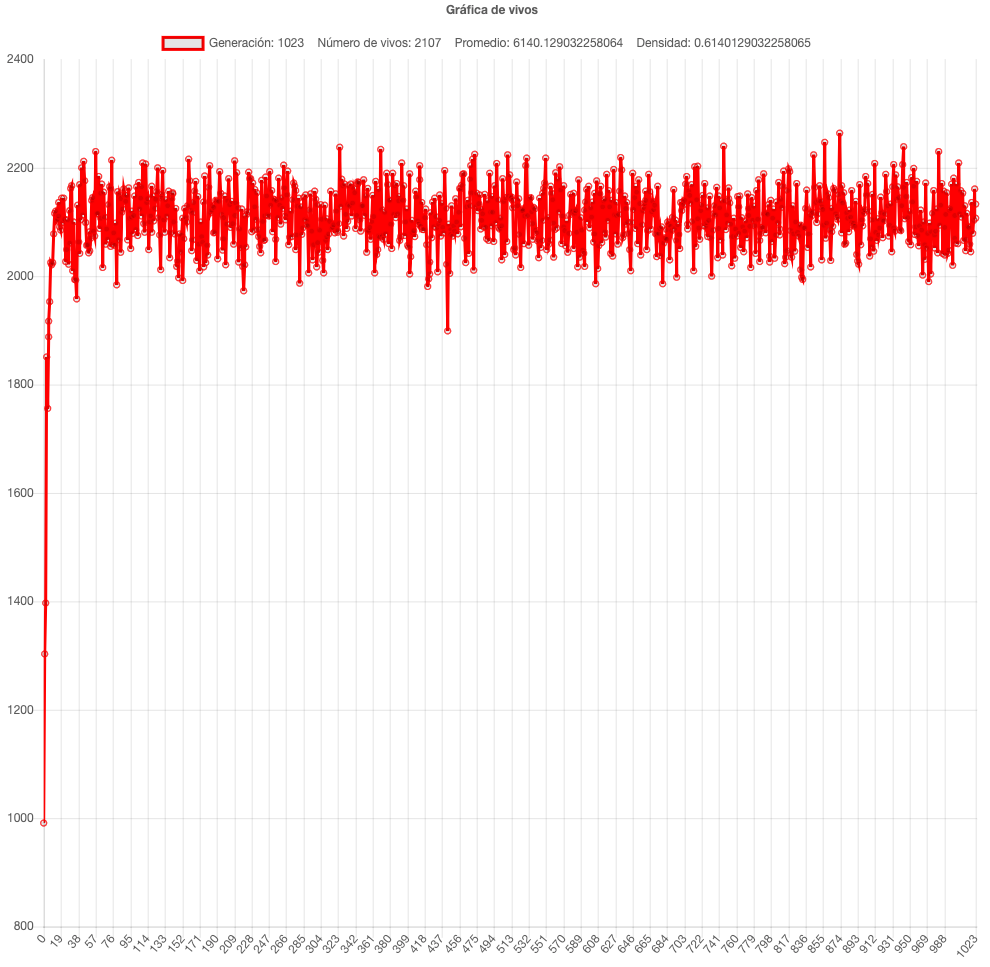
\includegraphics[scale=.24]{GOL/img/dif10-2.png}
			\caption{Comportamiento de la población de la simulación anterior}
			\label{fig:gol5}
		\end{center}
	\end{figure}

	\begin{figure}[H]
		\begin{center}
			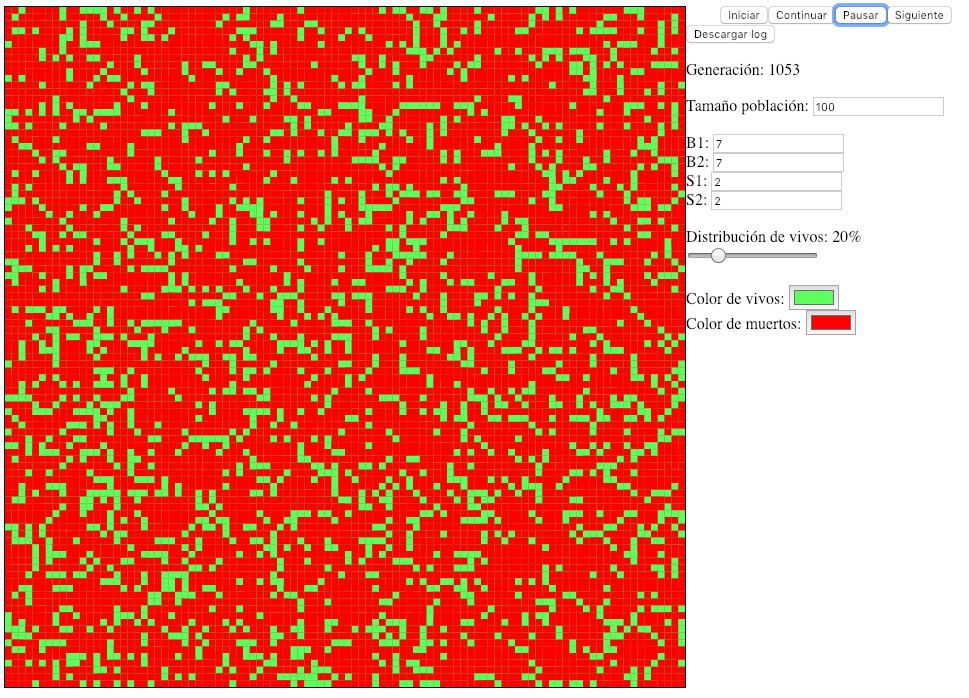
\includegraphics[scale=.3]{GOL/img/dif20-1.png}
			\caption{Regla de difusión con probabilidad de 20\%}
			\label{fig:gol5}
		\end{center}
	\end{figure}

	\begin{figure}[H]
		\begin{center}
			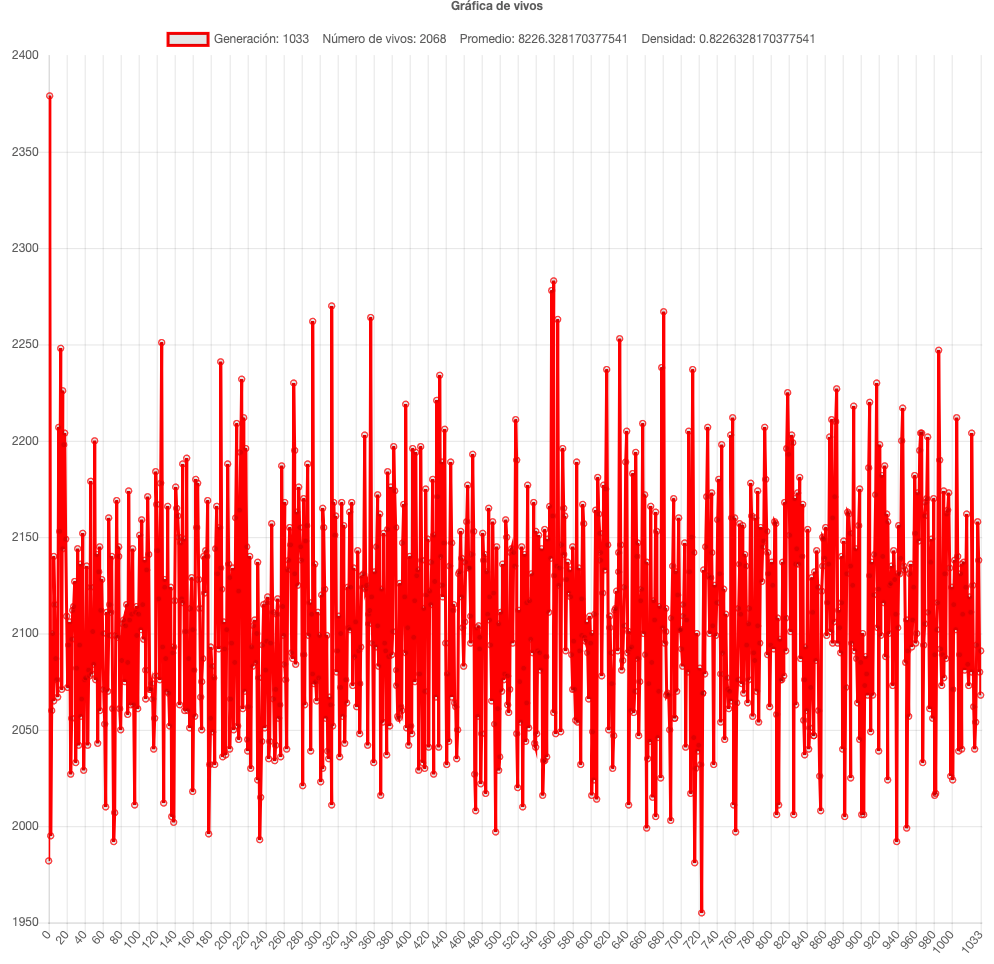
\includegraphics[scale=.24]{GOL/img/dif20-2.png}
			\caption{Comportamiento de la población de la simulación anterior}
			\label{fig:gol5}
		\end{center}
	\end{figure}

	\begin{figure}[H]
		\begin{center}
			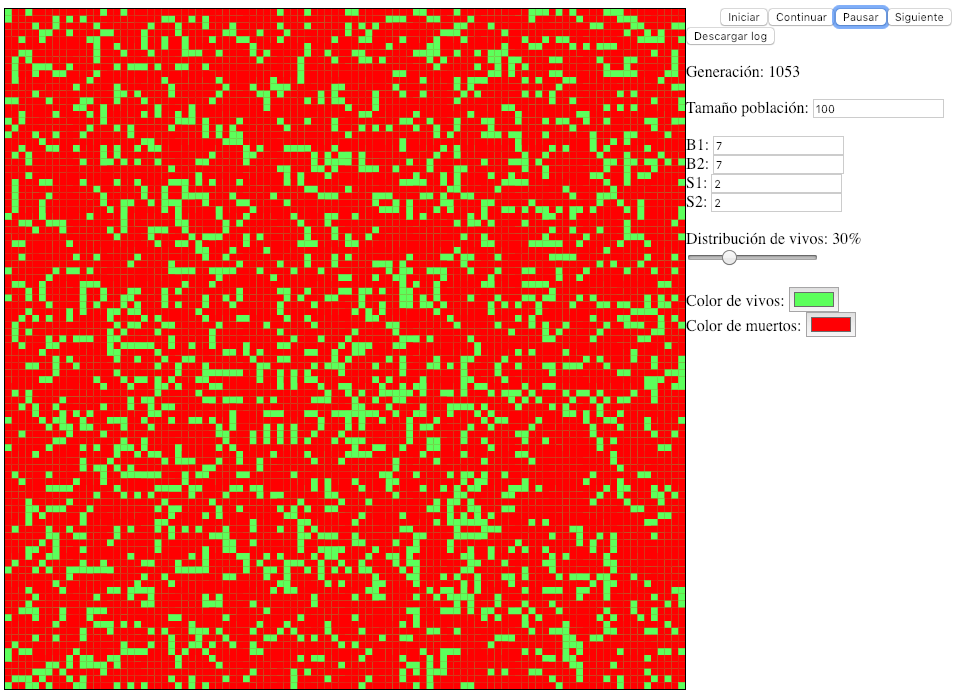
\includegraphics[scale=.3]{GOL/img/dif30-1.png}
			\caption{Regla de difusión con probabilidad de 30\%}
			\label{fig:gol5}
		\end{center}
	\end{figure}

	\begin{figure}[H]
		\begin{center}
			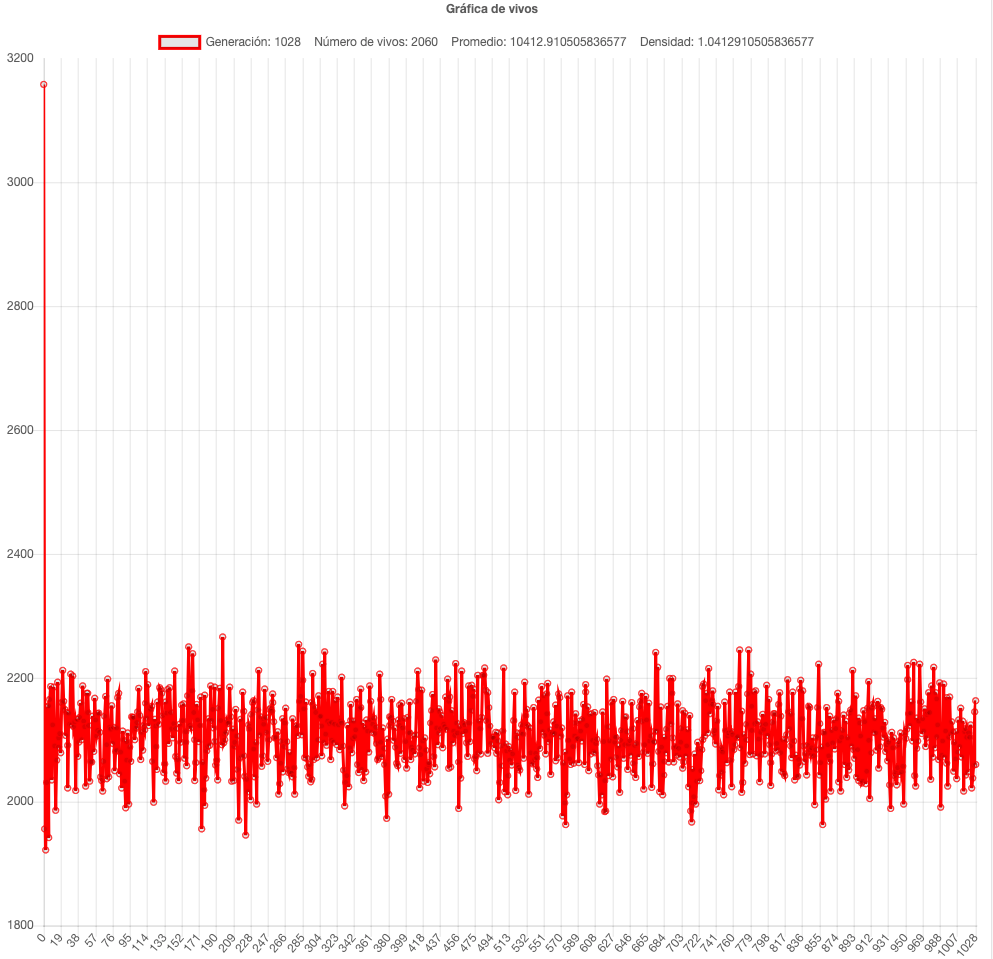
\includegraphics[scale=.24]{GOL/img/dif30-2.png}
			\caption{Comportamiento de la población de la simulación anterior}
			\label{fig:gol5}
		\end{center}
	\end{figure}

	\begin{figure}[H]
		\begin{center}
			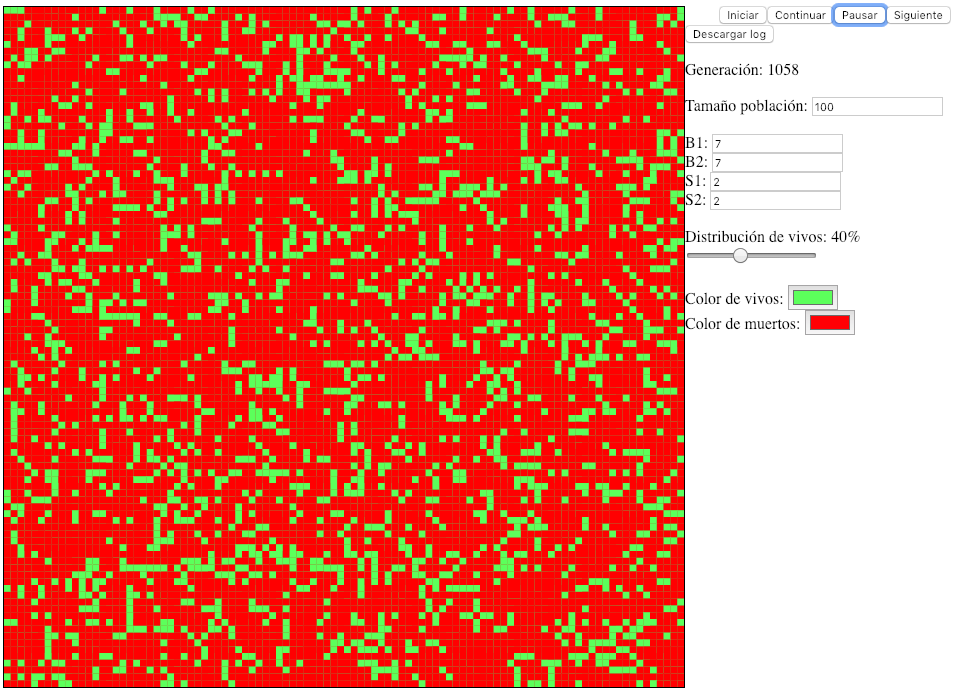
\includegraphics[scale=.3]{GOL/img/dif40-1.png}
			\caption{Regla de difusión con probabilidad de 40\%}
			\label{fig:gol5}
		\end{center}
	\end{figure}

	\begin{figure}[H]
		\begin{center}
			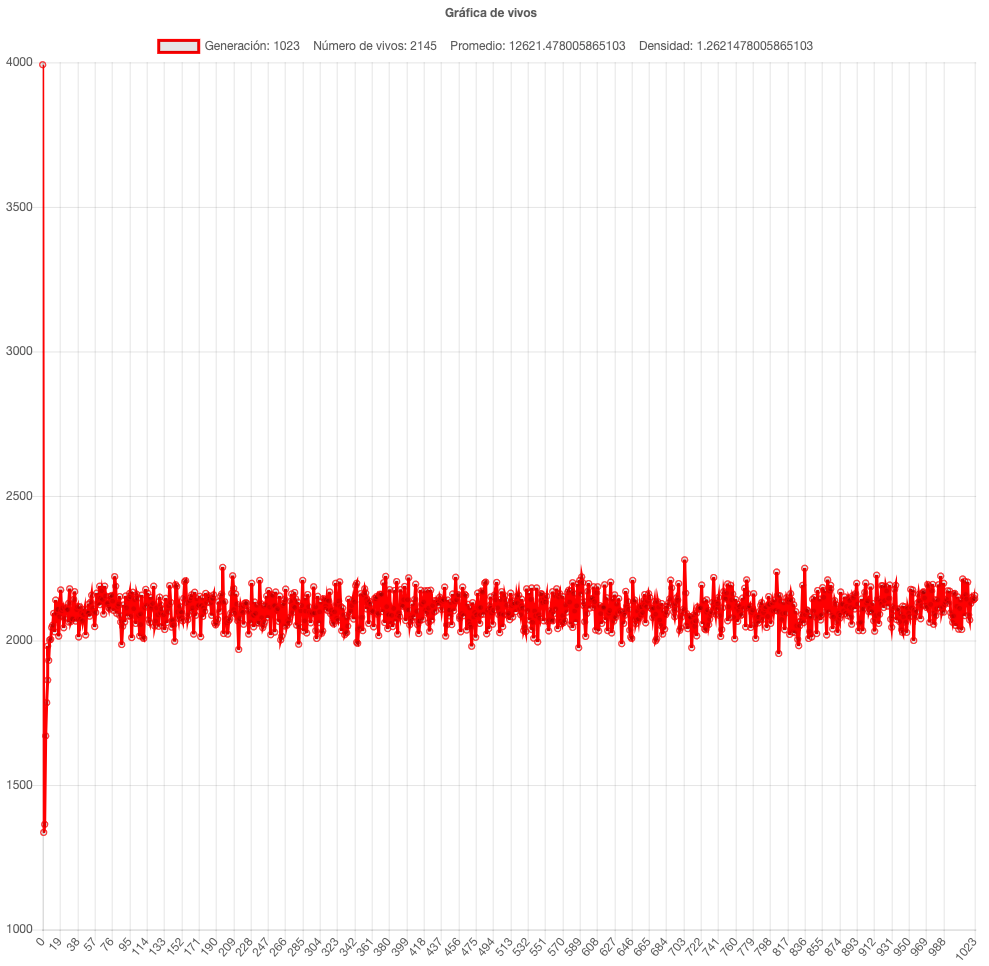
\includegraphics[scale=.24]{GOL/img/dif40-2.png}
			\caption{Comportamiento de la población de la simulación anterior}
			\label{fig:gol5}
		\end{center}
	\end{figure}

	\begin{figure}[H]
		\begin{center}
			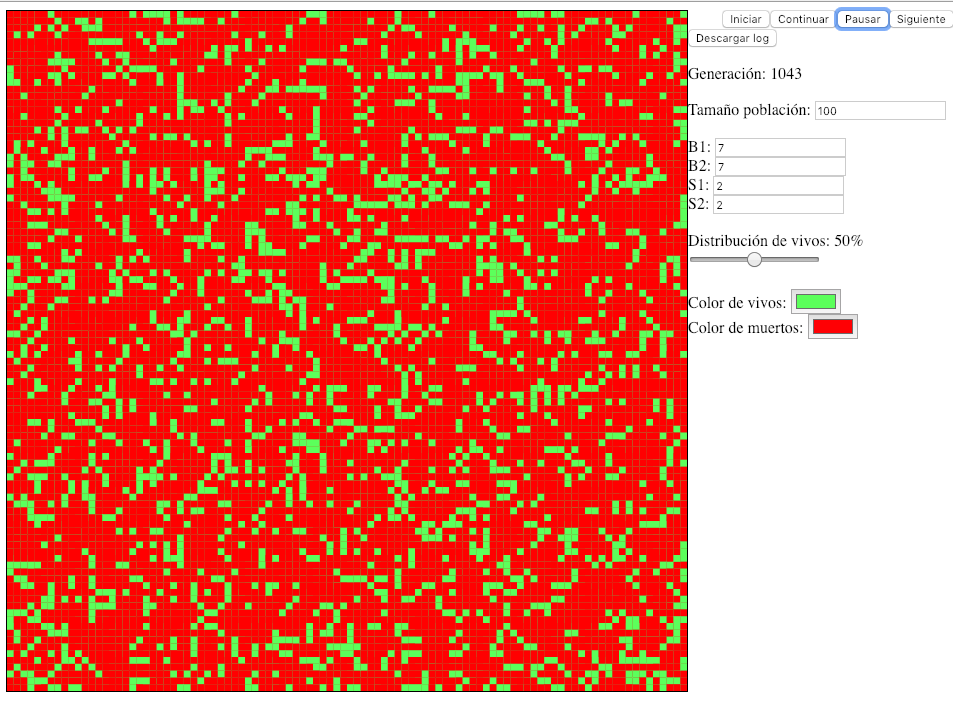
\includegraphics[scale=.3]{GOL/img/dif50-1.png}
			\caption{Regla de difusión con probabilidad de 50\%}
			\label{fig:gol5}
		\end{center}
	\end{figure}

	\begin{figure}[H]
		\begin{center}
			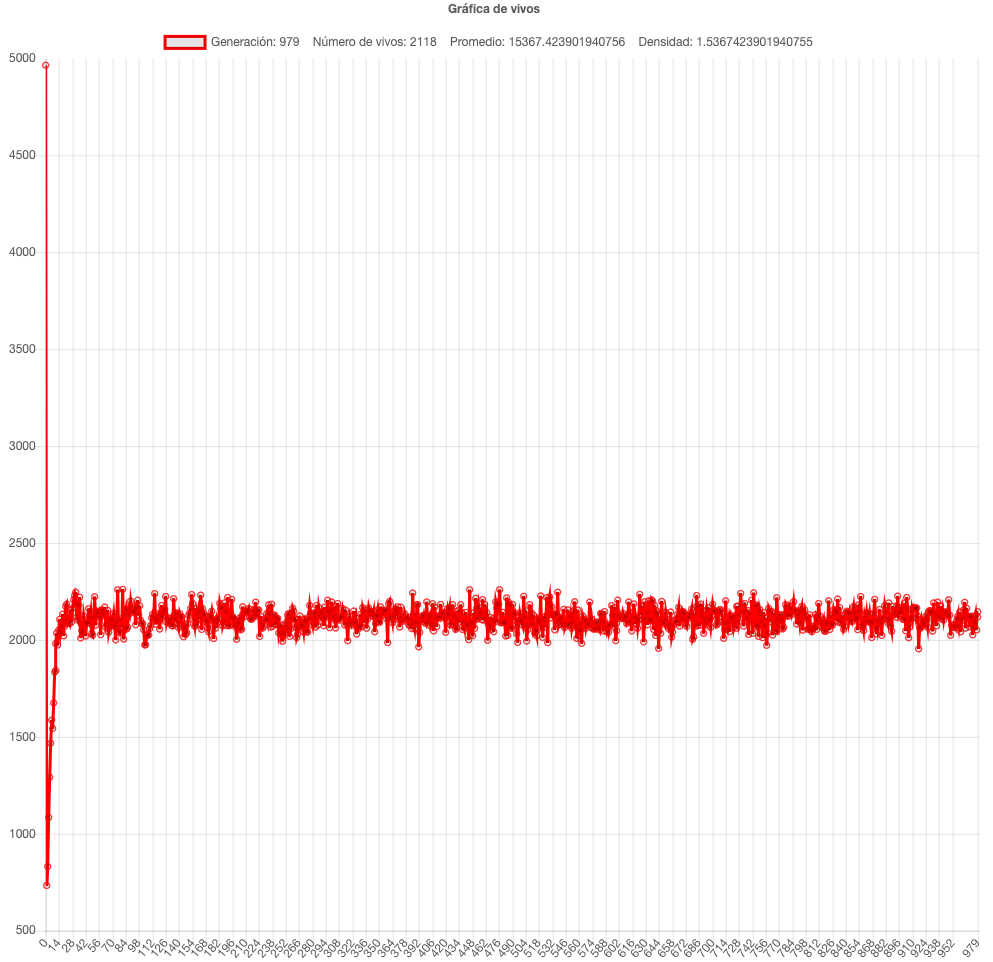
\includegraphics[scale=.24]{GOL/img/dif50-2.png}
			\caption{Comportamiento de la población de la simulación anterior}
			\label{fig:gol5}
		\end{center}
	\end{figure}

	\begin{figure}[H]
		\begin{center}
			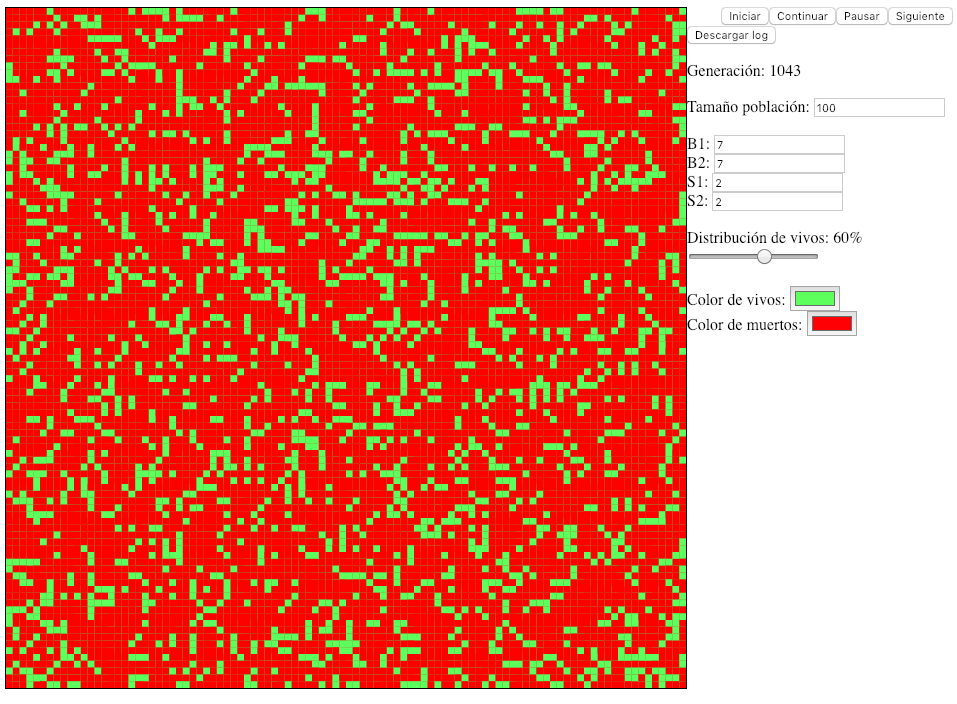
\includegraphics[scale=.3]{GOL/img/dif60-1.png}
			\caption{Regla de difusión con probabilidad de 60\%}
			\label{fig:gol5}
		\end{center}
	\end{figure}

	\begin{figure}[H]
		\begin{center}
			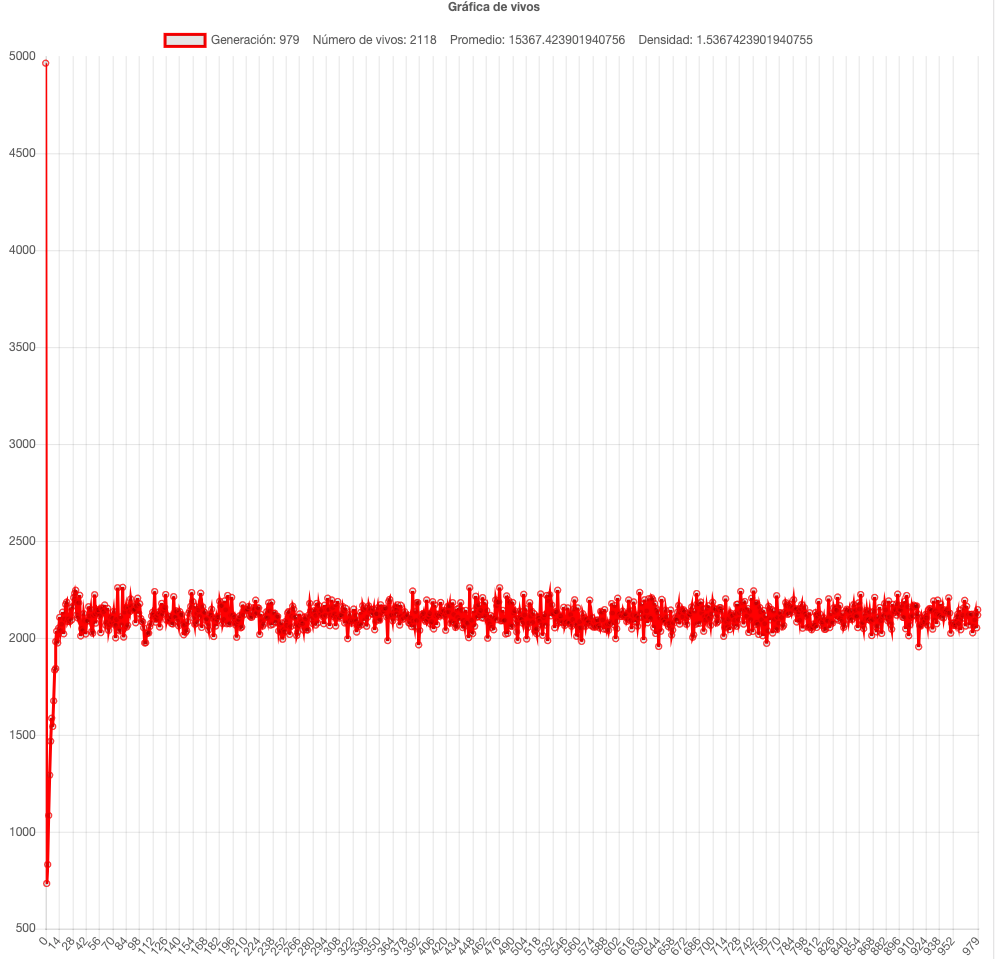
\includegraphics[scale=.24]{GOL/img/dif60-2.png}
			\caption{Comportamiento de la población de la simulación anterior}
			\label{fig:gol5}
		\end{center}
	\end{figure}

	\begin{figure}[H]
		\begin{center}
			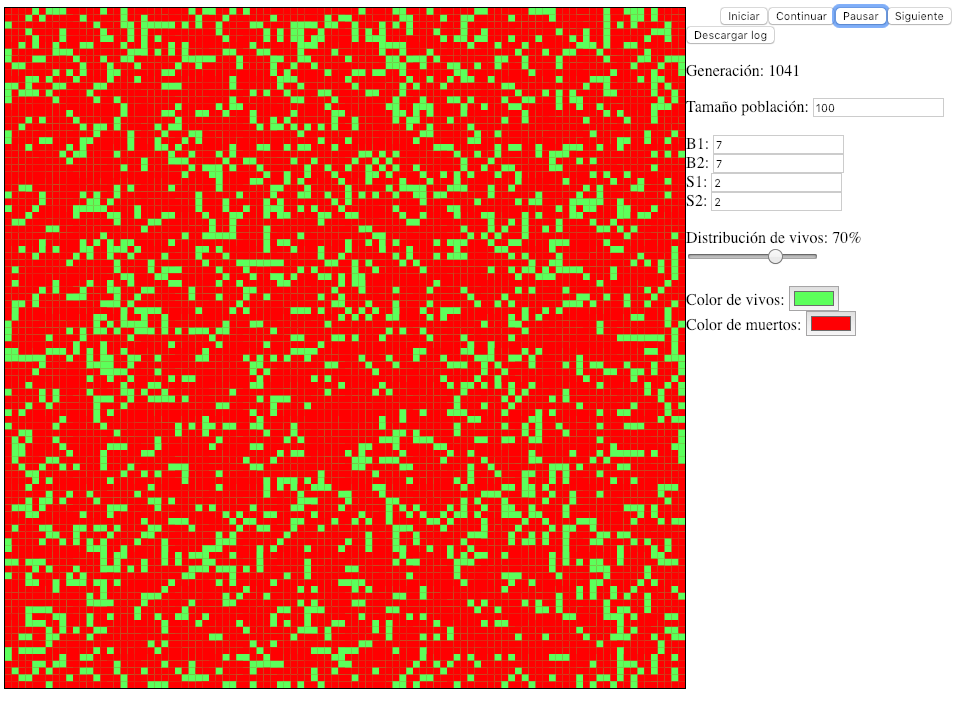
\includegraphics[scale=.3]{GOL/img/dif70-1.png}
			\caption{Regla de difusión con probabilidad de 70\%}
			\label{fig:gol5}
		\end{center}
	\end{figure}

	\begin{figure}[H]
		\begin{center}
			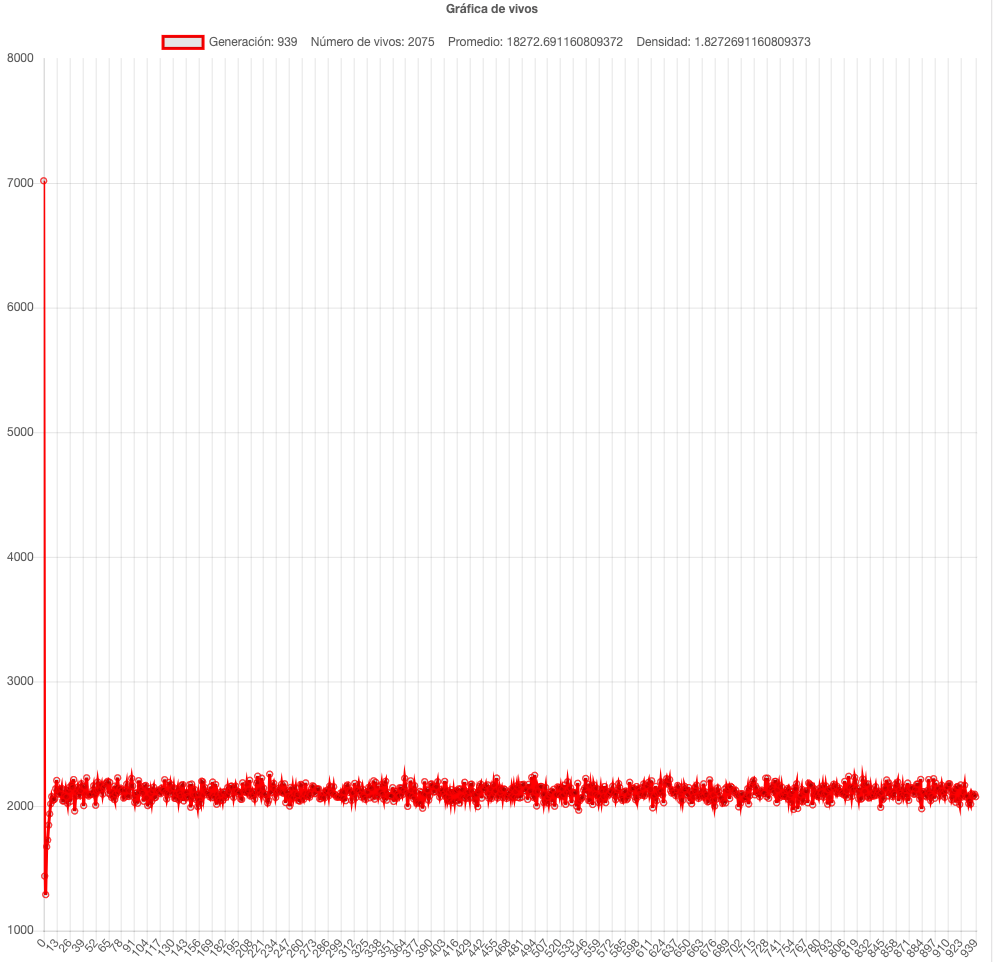
\includegraphics[scale=.24]{GOL/img/dif70-2.png}
			\caption{Comportamiento de la población de la simulación anterior}
			\label{fig:gol5}
		\end{center}
	\end{figure}

	\begin{figure}[H]
		\begin{center}
			\includegraphics[scale=.3]{GOL/img/dif80-1.png}
			\caption{Regla de difusión con probabilidad de 80\%}
			\label{fig:gol5}
		\end{center}
	\end{figure}

	\begin{figure}[H]
		\begin{center}
			\includegraphics[scale=.24]{GOL/img/dif80-2.png}
			\caption{Comportamiento de la población de la simulación anterior}
			\label{fig:gol5}
		\end{center}
	\end{figure}

	\begin{figure}[H]
		\begin{center}
			\includegraphics[scale=.3]{GOL/img/dif90-1.png}
			\caption{Regla de difusión con probabilidad de 90\%}
			\label{fig:gol5}
		\end{center}
	\end{figure}

	\begin{figure}[H]
		\begin{center}
			\includegraphics[scale=.24]{GOL/img/life90-2.png}
			\caption{Comportamiento de la población de la simulación anterior}
			\label{fig:gol5}
		\end{center}
	\end{figure}

Para la regla de difusión se podria decir que el comportamiento de la población es más estable que la de life, debido a que en todas las simulaciones la cantidad de vivos que se graficaban no era tan variable desde un inicio y el comportamiento de la gráfica es igual en todas las probabilidades de uno que se probaron en donde la población oscila entre un limite mayor y uno menor.
